\documentclass[12pt,openany]{book}

\usepackage{amsmath,amsthm,amsfonts,amscd} % Packages for mathematics
\usepackage{commath}

\usepackage{transparent}
% Colors
\usepackage[dvipsnames]{xcolor}
\definecolor{titleblue}{RGB}{0,53,128}
\definecolor{chaptergray}{RGB}{140,140,140}
\definecolor{sectiongray}{RGB}{180,180,180}

\definecolor{thmcolor}{RGB}{231, 76, 60}
\definecolor{defcolor}{RGB}{52, 152, 219}
\definecolor{lemcolor}{RGB}{155, 89, 182}
\definecolor{corcolor}{RGB}{46, 204, 113}
\definecolor{procolor}{RGB}{241, 196, 15}
\definecolor{execolor}{RGB}{90, 128, 127}

\usepackage{cancel}
\newcommand\crossout[3][black]{\renewcommand\CancelColor{\color{#1}}\cancelto{#2}{#3}}
\newcommand\ncrossout[2][black]{\renewcommand\CancelColor{\color{#1}}\cancel{#2}}
% Fonts
\usepackage[T1]{fontenc}
\usepackage[utf8]{inputenc}
\usepackage{newpxtext,newpxmath}
\usepackage{sectsty}
\allsectionsfont{\sffamily\color{titleblue}\mdseries}

% Page layout
\usepackage{geometry}
\geometry{a4paper,left=.8in,right=.6in,top=.75in,bottom=1in,heightrounded}
\usepackage{fancyhdr}
\fancyhf{}
\fancyhead[LE,RO]{\thepage}
\fancyhead[LO]{\nouppercase{\rightmark}}
\fancyhead[RE]{\nouppercase{\leftmark}}
\renewcommand{\headrulewidth}{0.5pt}
\renewcommand{\footrulewidth}{0pt}

% Chapter formatting
\usepackage{titlesec}
\titleformat{\chapter}[display]
{\normalfont\sffamily\Huge\bfseries\color{titleblue}}{\chaptertitlename\ \thechapter}{20pt}{\Huge}
\titleformat{\section}
{\normalfont\sffamily\Large\bfseries\color{titleblue!100!gray}}{\thesection}{1em}{}
\titleformat{\subsection}
{\normalfont\sffamily\large\bfseries\color{titleblue!75!gray}}{\thesubsection}{1em}{}

% Table of contents formatting
\usepackage{tocloft}
\renewcommand{\cftchapfont}{\sffamily\color{titleblue}\bfseries}
\renewcommand{\cftsecfont}{\sffamily\color{chaptergray}}
\renewcommand{\cftsubsecfont}{\sffamily\color{sectiongray}}
\renewcommand{\cftchapleader}{\cftdotfill{\cftdotsep}}

% Hyperlinks
\usepackage{hyperref}
\hypersetup{
	colorlinks=true,
	linkcolor=titleblue,
	filecolor=black,      
	urlcolor=titleblue,
}

%Ceiling and Floor Function
\usepackage{mathtools}
\DeclarePairedDelimiter{\ceil}{\lceil}{\rceil}
\DeclarePairedDelimiter{\floor}{\lfloor}{\rfloor}

%Algorithm
\usepackage[ruled,linesnumbered]{algorithm2e}
\usepackage{setspace}
\usepackage{algpseudocode}
\SetKwComment{Comment}{/* }{ */}
\SetKw{Break}{break}
\SetKw{Downto}{downto}
\SetKwProg{Fn}{Function}{:}{end}
\SetKwFunction{KeyGen}{KeyGen}


%---------------------------My Preamble
\usepackage{marvosym} %Lightning
\usepackage{booktabs}
\usepackage{multicol}
\setlength{\columnsep}{2cm}
\setlength{\columnseprule}{1.25pt}
\usepackage{enumerate}
\usepackage{soul}
\newcommand{\mathcolorbox}[2]{\colorbox{#1}{$\displaystyle #2$}}
\usepackage{graphicx}
\usepackage{tikz}
\usepackage{tikz-cd}
\usetikzlibrary{patterns, patterns.meta}
\usetikzlibrary{calc}
\usetikzlibrary{arrows, arrows.meta, positioning, shapes.multipart}
\usepackage{pgfplots}
\usepackage{mathrsfs}

%Tcolorbox
\usepackage[most]{tcolorbox}
\tcbset{colback=white, arc=5pt}
%\tcbset{enhanced, colback=white,colframe=black,fonttitle=\bfseries,arc=4mm,boxrule=1pt,shadow={2mm}{-1mm}{0mm}{black!50}}
%White box with black text and shadow
%\begin{tcolorbox}[colback=white,colframe=black,fonttitle=\bfseries,title=Black Shadow Box,arc=4mm,boxrule=1pt,shadow={2mm}{-1mm}{0mm}{black!50}]
%	This is a white box with black text and a subtle shadow. The shadow adds some depth and dimension to the box without overpowering the design.
%\end{tcolorbox}

%Theorem
\newtheorem{axiom}{Axiom}[chapter]
\newtheorem{theorem}{Theorem}[chapter]
\newtheorem{proposition}[theorem]{Proposition}
\newtheorem{corollary}{Corollary}[theorem]
\newtheorem{lemma}[theorem]{Lemma}

\theoremstyle{definition}
\newtheorem{definition}{Definition}[chapter]
\newtheorem{remark}{Remark}[chapter]
\newtheorem{exercise}{Exercise}[chapter]
\newtheorem{example}{Example}[chapter]
\newtheorem*{note}{Note}

%New Command
\newcommand{\N}{\mathbb{N}}
\newcommand{\Z}{\mathbb{Z}}
\newcommand{\Q}{\mathbb{Q}}
\newcommand{\R}{\mathbb{R}}
\newcommand{\C}{\mathbb{C}}
\newcommand{\F}{\mathbb{F}}

\newcommand{\ie}{\textnormal{i.e.}}
\newcommand{\eg}{\textnormal{e.g.}}

\newcommand{\of}[1]{\left( #1 \right)} 

\newcommand{\nbhd}{\mathcal{N}}
\newcommand{\Id}{\operatorname{\textnormal{id}}}

\newcommand{\sol}{\textcolor{magenta}{\bf Solution}}

\newcommand{\Caratheodroy}{Carath\'{e}odory}

\newcommand{\upRiemannint}[2]{
	\overline{\int_{#1}^{#2}}
}
\newcommand{\loRiemannint}[2]{
	\underline{\int_{#1}^{#2}}
}

\newcommand{\inner}[1]{\left\langle #1 \right\rangle}

% Begin document
\begin{document}
	
	% Title page
	\begin{titlepage}
		\begin{center}
			{\Huge\textsf{\textbf{Introduction to Applied Mathematics}}\par}
			{\Huge\textsf{\textbf{- Advance Calculus II -}}\par}
			\vspace{0.5in}
			{\Large Ji Yong-Hyeon\par}
			\vspace{1in}
			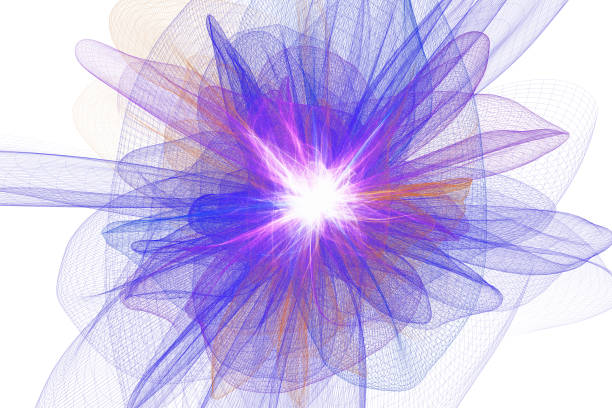
\includegraphics[scale=3]{iam2.jpg}\par
			\vspace{1in}
			{\large\bf Department of Information Security, Cryptology, and Mathematics\par}
			{College of Science and Technology\par}
			{Kookmin University\par}
			%\includegraphics[width=1.5in]{school_logo.jpg}\par
			\vspace{.25in}
			{\large \today\par}
		\end{center}
	\end{titlepage}
	
	% Table of contents
	\tableofcontents
	
	% Chapters
	\mainmatter
	
	\chapter{Differentiation}
	\section{Derivative and \Caratheodroy's Theorem}
	\begin{tcolorbox}[colback=white,colframe=defcolor,arc=5pt,title={\color{white}\bf Derivative}]
		\begin{definition}
			Let $f:I\to\R$ and $a\in I$. We say that $L\in\R$ is the \textbf{derivative of} $f$ at $a$ if \[
			\forall\epsilon>0:\exists\delta>0:x\in\nbhd_\delta^*(a)\cap I\implies\abs{\frac{f(x)-f(a)}{x-a}-L}<\epsilon.
			\]
		\end{definition}
	\end{tcolorbox}
	\begin{remark}
		We say that $f$ is \textbf{differentiable} at $a$, and we write $L=f'(a)$. In other words, $\displaystyle f'(a)=\lim\limits_{x\to a} \frac{f(x)-f(a)}{x-a}$.
	\end{remark}
	\vspace{8pt}
	\begin{tcolorbox}[colback=white,colframe=procolor,arc=5pt,title={\color{white}\bf }]
		\begin{proposition}
			If $f:I\to\R$ has a derivative at $a\in I$ then $f$ is continuous at $a$. That is, \[
			\exists f'(a)\implies f(a)=\lim\limits_{x\to a}f(x).
			\]
		\end{proposition}
	\end{tcolorbox}
	\begin{proof}
		Let $\exists f'(a)$. Then \begin{align*}
			\lim\limits_{x\to a} [f(x)-f(a)]&=\lim\limits_{x\to a}\left[\frac{f(x)-f(a)}{x-a}\cdot (x-a)\right]\quad\because x\in\nbhd_\delta^*(a)\Rightarrow x\neq a\\
			&=\lim\limits_{x\to a}\frac{f(x)-f(a)}{x-a}\lim\limits_{x\to a}(x-a)\\
			&=f'(a)\cdot 0=0.
		\end{align*}
	\end{proof}
	\vspace{4pt}
	\begin{remark}
		The continuity of $f:I\to\R$ at point does not assure the existence of the derivative at that point, \eg, $f(x):=\abs{x}$ for $x\in\R$.
	\end{remark}
	
	\begin{tcolorbox}[colback=white,colframe=thmcolor,arc=5pt,title={\color{white}\bf $\star$ \Caratheodroy's Theorem $\star$}]
		\begin{theorem}
			Let $f$ be defined on an interval $I$ containing the point $a$. Then \[
			\exists f'(a)\iff\exists\varphi\in\R^I\quad\textnormal{such that}\quad
			\begin{cases}
				\textnormal{$\varphi$ is continuous on $I$}&\cdots\textnormal{(1)}\\
				\\
				f(x)-f(a)=\varphi(x)(x-a)&\cdots\textnormal{(2)}
			\end{cases}
			\] In this case, we have $\varphi(a)=f'(a)$.
		\end{theorem}
	\end{tcolorbox}
	\begin{proof}
		\begin{itemize}
			\item[($\Rightarrow$)] Assume that $\exists f'(a)$. Define a function $\varphi:I\to\R$ as following \[
			\varphi(x)=\begin{cases}
				\displaystyle\frac{f(x)-f(a)}{x-a} &:x\neq a\\
				\\
				f'(a) &:x=a.
			\end{cases}
			\] Then \begin{enumerate}[(i)]
				\item $\phi$ is continuous on $I$, \ie, for all $a\in I$, $$\lim\limits_{x\to a}\varphi(x)=\lim\limits_{x\to a}\frac{f(x)-f(a)}{x-a}=f'(a)=\varphi(a).$$
				\item \[
				\begin{cases}
					f(x)-f(a)=\varphi(x)(x-a) &: x\neq a\\
					0=\varphi(x)\cdot 0 &: x=a.
				\end{cases}
				\]
			\end{enumerate}
			\item[($\Leftarrow$)] Let $x\neq a$ and $x\to a$. The continuity of $\varphi$ gives that \[
			\exists\phi(a)=\lim\limits_{x\to a}\varphi(x)=\lim\limits_{x\to a}\frac{\varphi(x)(x-a)}{(x-a)}=\lim\limits_{x\to a}\frac{f(x)-f(a)}{x-a}=f'(a).
			\] That is, $f$ is differentiable at $a$ and $f'(a)=\varphi(a)$.
		\end{itemize}
	\end{proof}
	\vspace{4pt}
	\begin{example}
		Let us consider the function $f$ defined by $f(x):=x^3$ for $x\in\R$. For any $a\in\R$, we see from the factorization \[
		f(x)-f(a)=x^3-a^3=(x^2+ax+a^2)(x-a)
		\] that $\varphi(x):=x^2+ax+a^2$ satisfies the condition of \Caratheodroy's Theorem. Therefore, we conclude that $f$ is differentiable at $a\in\R$ and that $f'(a)=\varphi(a)=3a^2$.
	\end{example}
	
	\newpage
	\begin{tcolorbox}[colback=white,colframe=thmcolor,arc=5pt,title={\color{white}\bf Chain Rule}]
		\begin{theorem}
			Let $I,J$ be intervals in $\R$, let $g:J\to\R$ and $f:I\to\R$ be functions such that $f[I]\subseteq J$, and let $a\in I$. Then \[
			\exists f'(a)\exists g'(f(a))\implies\exists(g\circ f)'(a)
			\] and $(g\circ f)'(a)=g'(f(a))f'(a)$.
		\end{theorem}
	\end{tcolorbox}
	\begin{proof}
		We must show that there exists a continuous function $\varphi(x)$ s.t. \[
		g(f(x))-g(f(a))=\varphi(x)(x-a).
		\]
		\begin{enumerate}[(1)]
			\item Since $\exists f'(a)$, by \Caratheodroy's Theorem, $\exists\sigma:I\to\R$ s.t. \begin{enumerate}[(i)]
				\item $\sigma$ is continuous at $a\in I$;
				\item $f(x)-f(a)=\sigma(x)(x-a)$;
				\item $f'(a)=\sigma(a)$.
			\end{enumerate}
			\item Since $\exists g'(f(a))$, by \Caratheodroy's Theorem, $\exists\tau:J\to\R$ s.t. \begin{enumerate}[(i)]
				\item $\tau$ is continuous at $f(a)\in J$;
				\item $g(f(x))-g(f(a))=\tau(f(x))(f(x)-f(a))$;
				\item $g'(f(a))=\tau(f(a))$.
			\end{enumerate}
		\end{enumerate} Then \begin{align*}
			g(f(x))-g(f(a))&=\tau(f(x))(f(x)-f(a))\quad\text{by (2)-(ii)}\\
			&=\tau(f(x))\sigma(x)(x-a)\quad\text{by (1)-(ii)}.
		\end{align*} Let $\varphi(x):=\tau(f(x))\sigma(x)$. Then \begin{enumerate}[(i)]
			\item $\phi:I\to\R$ is continuous at $a$ and
			\item $g(f(x))-g(f(a))=\varphi(x)(x-a)$,
		\end{enumerate} and so, by \Caratheodroy's Theorem, \[
		\exists(g\circ f)'(a)=\varphi(a)=\tau(f(a))\cdot \sigma(a)=g'(f(a))\cdot f'(a).
		\]
	\end{proof}
	\vspace{4pt}
	\begin{remark}
		If $f$ is a differentiable function, then the chain rule implies that the function $g\circ f=\abs{f}$ is also differentiable at all points $x$ where $f(x)\neq 0$, and its derivative is given by \[
		\abs{f(x)}'(x)=\mathsf{sgn}(f(x))\cdot f'(x)=\begin{cases}
			f'(x) &:f(x)>0,\\
			-f'(x) &:f(x)<0.
		\end{cases}
		\]
	\end{remark}
	\vspace{4pt}
	\begin{remark}\it
		A function $f$ that is differentiable at every point of $\R$ \textbf{need not} have a continuous derivative $f'$.
	\end{remark}
	
	\newpage
	\begin{tcolorbox}[colback=white,colframe=thmcolor,arc=5pt,title={\color{white}\bf Differentiablility of The Inverse Function}]
		\begin{theorem}
			Let $f:I\to\R$ be strictly monotone and continuous on $I$. Let $J:=f[I]$ and $g:J\to\R$ be the strictly monotone and continuous function inverse to $f$. Then \[
			\exists f'(a)\neq 0\implies\exists g'(f(a))=\frac{1}{f'(a)}.
			\]
		\end{theorem}
	\end{tcolorbox}
	\begin{proof}
		Since $\exists f'(a)$, by \Caratheodroy's Theorem, $\exists\sigma:I\to\R$ s.t. \begin{enumerate}[(i)]
			\item $\sigma$ is continuous at $a\in I$;
			\item $f(x)-f(a)=\sigma(x)(x-a)$;
			\item $f'(a)=\sigma(a)\neq 0$.
		\end{enumerate} Since $\sigma(a)\neq 0$, $\exists\delta>0$ s.t. $\sigma(x)\neq0$, $x\in\nbhd_\delta(a)\cap I$.
		Let $\Omega:=f[\nbhd_\delta(a)\cap I]$. Since $g=f^{-1}$, we have \begin{align*}
			f(\textcolor{red}{x})-f(\textcolor{blue}{a})&=f(\textcolor{red}{(g\circ f)(x)})-f(\textcolor{blue}{(g\circ f)(a)})\quad\because f\circ g=\Id\\
			&=\sigma(\textcolor{red}{(g\circ f)(x)})(\textcolor{red}{(g\circ f)(x)}-\textcolor{blue}{(g\circ f)(a)})\quad\text{by (ii)}.
		\end{align*} Since $f(x)\in\Omega\Rightarrow\sigma(x)\neq 0\Rightarrow \sigma((g\circ f)(x))\neq 0$, \[
		g(f(x))-g(f(a))=\frac{1}{\sigma((g\circ f)(x))}(f(x)-f(a)).
		\] Let $\varphi(x):=1/\sigma((g\circ f)(x))$. Then $\varphi$ is continuous at $f(a)$. By \Caratheodroy's Theorem, \[
		g'(f(a))=\varphi(a)=\frac{1}{\sigma((g\circ f)(a))}=\frac{1}{\sigma(a)}=\frac{1}{f'(a)}.
		\]
	\end{proof}
	
	\newpage
	\section{The Rolle's Theorem and the Mean Value Theorem}
	\begin{tcolorbox}[colback=white,colframe=defcolor,arc=5pt,title={\color{white}\bf Absolute and Local Maxi/Mini-mum}]
		\begin{definition}
			Let $f:I\to\R$ be a function.
			\begin{itemize}
				\item $f$ has an \textbf{absolute maximum} at $a\in I$ if $x\in I\implies f(x)\leq f(a)$.
				\item $f$ has an \textbf{absolute minimum} at $a\in I$ if $x\in I\implies f(a)\leq f(x)$.
				\item $f$ is said to have a \textbf{local (or relative) maximum} at $a\in I$ if \[
				\exists\nbhd_\delta(a):f(x)\leq f(a),\ x\in\nbhd_\delta(a)\cap I.
				\]
				\item $f$ is said to have a \textbf{local (or relative) minimum} at $a\in I$ if \[
				\exists\nbhd_\delta(a):f(a)\leq f(x),\ x\in\nbhd_\delta(a)\cap I.
				\]
				\item $f$ has a \textbf{local (or relative extremum)} at $a\in I$ either a relative maximum or a relative minimum at $a$.
			\end{itemize}
		\end{definition}
	\end{tcolorbox}
	\vspace{8pt}
	\begin{tcolorbox}[colback=white,colframe=thmcolor,arc=5pt,title={\color{white}\bf Interior Extremum Theorem}]
		\begin{theorem}
		Let $f:(a,b)\to\R$ has a relative extremum and $c\in(a,b)$. Then \[
		\exists f'(c)\implies f'(c)=0.
		\]
		\end{theorem}
	\end{tcolorbox}
	\begin{proof}
		Let $f$ has a relative maximum at $c$, \ie, \[
		\exists\nbhd_\delta(a): x\in\nbhd_\delta(a)\cap (a,b)\implies f(x)\leq f(a).
		\] Assume that $f'(c)>0$ then \[
		\exists\nbhd_\delta(c)\subseteq(a,b):x\in\nbhd_\delta^*(c)\Rightarrow\frac{f(x)-f(c)}{x-c}>0.
		\] If $c\in\nbhd_\delta(c)$ and $x>c$, then we have \[
		f(x)-f(c)=(x-c)\cdot\frac{f(x)-f(c)}{x-c}>0.
		\] But this contradicts the hypothesis that $f$ has a relative maximum at $c$. Similarly if $f'(c)<0$ then we have a contradiction. Hence $f'(c)=0$.
	\end{proof}
	\vspace{4pt}
	\begin{tcolorbox}[colback=white,colframe=corcolor,arc=5pt,title={\color{white}\bf }]
		\begin{corollary}
			Let $f:(a,b)\to\R$ be continuous on $(a, b)$ and suppose that $f$ has a relative
			extremum at $c\in(a, b)$. Then either \[
			\nexists f'(c)\quad\text{or}\quad f'(c)=0.
			\]
		\end{corollary}
	\end{tcolorbox}
	\vspace{8pt}
	
	\begin{tcolorbox}[colback=white,colframe=thmcolor,arc=5pt,title={\color{white}\bf $\star$ Rolle's Theorem}]
		\begin{theorem}
			Let $f$ is continuous on $I = [a, b]$, and let $f$ is differentiable on $(a,b)$. Then \[
			f(a)=0=f(b)\implies\exists c\in(a,b):f'(c)=0.
			\]
		\end{theorem}
	\end{tcolorbox}
	\vspace{8pt}
	\begin{tcolorbox}[colback=white,colframe=thmcolor,arc=5pt,title={\color{white}\bf $\star$ Mean Value Theorem of Differential Calculus $\star$}]
		\begin{theorem}
			Let $f$ is continuous on $I = [a, b]$, and let $f$ is differentiable on $(a,b)$. Then \[
			\exists c\in(a,b):f(b)-f(a)=f'(c)(b-a).
			\]
		\end{theorem}
	\end{tcolorbox}
	\begin{proof}
		Consider the function whose graph is the line segment joining the points \((a,f(a))\) and \((b,f(b))\): \[
		f(x)-f(a)=\frac{f(b)-f(a)}{b-a}(x-a).
		\] Define a function \(g:[a,b]\to\R\) s.t. \[
		g(x):=f(x)-f(a)-\frac{f(b)-f(a)}{b-a}(x-a)
		\] Then \begin{enumerate}[(i)]
			\item \(g\) is continuous on \([a,b]\);
			\item \(g\) is differentiable on \((a,b)\);
			\item \(g(a)=0=g(b)\). 
		\end{enumerate} By Rolle's Theorem, \(\exists c\in(a,b):g'(c)=0\). Then \[
		g'(x)=f'(x)-\frac{f(b)-f(a)}{b-a}\implies g'(c)=f'(c)-\frac{f(b)-f(a)}{b-a}=0\implies
		f'(c)=\frac{f(b)-f(a)}{b-a}.
		\]
	\end{proof}
	\vspace{8pt}
	\begin{example}
		Prove that $e^x\geq 1+x$ for $x\in\R$.
		\begin{proof}[\sol]
			\begin{enumerate}[(1)]
				\item \(x=0\implies e^x=1+x\).
				\item Let \(x>0\) and \(f(x)=e^x\). Then, by MVT, \[
				\exists c\in(0,x):f(x)-f(0)=f'(c)(x-0),
				\] and so \[
				e^x-1=e^cx> x\implies e^x>1+x.
				\]
				\item Let $x<0$ and $f(x)=e^x$. Then, by MVT, \[
				\exists c\in(x,0): f(0)-f(x)=f'(c)(0-x),
				\] and so \[
				1-e^x=e^c(-x)< -x\implies 1+x<e^x.
				\]
			\end{enumerate}
		\end{proof}
	\end{example}
	\newpage
	\section{L'H\^{o}spital's Rules}
	\begin{tcolorbox}[colback=white,colframe=thmcolor,arc=5pt,title={\color{white}\bf }]
		\begin{theorem}
			Let $f$ and $g$ be defined on $[a,b]$, let $f(a)=0=g(a)$, and let $g(x)\neq 0$ for $x\in(a,b)$. If $f$ and $g$ are differentiable at $a$ if $g'(a)\neq 0$, then the limit $f/g$ at a exits and is equal to $f'(a)/g'(a)$. Thus \[
			\lim\limits_{x\to a+}\frac{f(x)}{g(x)}=\frac{f'(a)}{g'(a)}.
			\]
		\end{theorem}
	\end{tcolorbox}
	\begin{proof}
		Since $f(a)=0=g(a)$, \[
		\lim\limits_{x\to a+}\frac{f(x)}{g(x)}=\lim\limits_{x\to a+}\frac{f(x)-f(a)}{g(x)-f(a)}=\lim\limits_{x\to a+}\frac{\frac{f(x)-f(a)}{x-a}}{\frac{g(x)-f(a)}{x-a}}=\frac{f'(a)}{g'(a)}.
		\]
	\end{proof}
	\vspace{10pt}
	\begin{remark}
		In L'H\^{o}spital Rules, the hypothesis $f(a)=0=g(a)$ is essential. For example, it $f(x):=x+17$ and $g(x):=2x+3$ for $x\in\R$ then, \[
		\lim\limits_{x\to 0}\frac{f(x)}{g(x)}=\frac{17}{3}\quad\text{while}\quad\frac{f'(0)}{g'(0)}=\frac{1}{2}.
		\]
	\end{remark}
	\vspace{20pt}
	\begin{tcolorbox}[colback=white,colframe=thmcolor,arc=5pt,title={\color{white}\bf Cauchy's Mean Value Thoerem of Differential Calculus}]
		\begin{theorem}
			Let $f$ and $g$ be continuous on $[a,b]$ and differentiable on $(a,b)$, and assume that $g'(x)\neq 0$ for all $x\in(a,b)$. Then \[
			\exists c\in(a,b):\frac{f(b)-f(a)}{g(b)-g(a)}=\frac{f'(c)}{g'(c)}.
			\]
		\end{theorem}
	\end{tcolorbox}
	\begin{proof}
		Since $g'(x)\neq 0$ for $x\in (a,b)$, $g(a)\neq g(b)$ by Rolle's Theorem. Define $h:[a,b]\to\R$ such that \[
		h(x):=f(x)-g(a)-\frac{f(b)-f(a)}{g(b)-g(a)}\del{g(x)-g(a)}.
		\] Then \begin{enumerate}[(i)]
			\item $h$ is continuous on $[a,b]$;
			\item $h$ is differentiable on $(a,b)$;
			\item $h(a)=0=h(b)$.
		\end{enumerate} By Rolle's Theorem, \[
		\exists c\in(a,b):h'(c)=0.
		\] Since $h'(x)=f'(x)-\frac{f(b)-f(a)}{g(b)-g(a)}g'(x)$, we have \[
		0=h'(c)=f'(c)-\frac{f(b)-f(a)}{g(b)-g(a)}g'(c)\implies\frac{f(b)-f(a)}{g(b)-g(a)}=\frac{f'(c)}{g'(c)}.
		\]
	\end{proof}
	\begin{remark}
		Note that if $g(x):=x$ then the Cauchy's mean value theorem reduces to the mean value theorem.
	\end{remark}
	\begin{remark}
		By the Mean Value Theorem, \[
		\exists \alpha,\beta\in(a,b):\begin{cases}
			f(b)-f(a)=f'(\alpha)(b-a)\\
			\\
			f(b)-f(a)=g'(\beta)(b-a)
		\end{cases}.
		\] If $g'(x)\neq 0$ for $x\in(a,b)$, we have $\displaystyle
		\frac{f(b)-f(a)}{g(b)-g(a)}=\frac{f'(\alpha)}{g'(\beta)}.
		$
	\end{remark}
	\vspace{20pt}
	\begin{tcolorbox}[colback=white,colframe=thmcolor,arc=5pt,title={\color{white}\bf L'H\^{o}pital's Rule - 1st}]
		\begin{theorem}
			Let $-\infty\leq a<b\leq\infty$ and let $f,g$ be differentiable on $(a,b)$ such that $g'(x)\neq 0$ for all $x\in(a,b)$. Suppose that \[
			\lim\limits_{x\to a+}f(x)=0=\lim\limits_{x\to a+}g(x).
			\] Then \begin{enumerate}[(1)]
				\item $\displaystyle\lim\limits_{x\to a+}\frac{f'(x)}{g'(x)}=L\implies\lim\limits_{x\to a+}\frac{f(x)}{g(x)}=L$.
				\item $\displaystyle\lim\limits_{x\to a+}\frac{f'(x)}{g'(x)}=\pm\infty\implies\lim\limits_{x\to a+}\frac{f(x)}{g(x)}=\pm\infty$.
			\end{enumerate}
		\end{theorem}
	\end{tcolorbox}
	\begin{proof}
		We must show that $\lim\limits_{x\to a+}\frac{f(x)}{g(x)}=L$, \ie, 
		\begin{align*}
			&\forall\varepsilon>0:\exists\delta>0:x\in(a,a+\delta)\implies\abs{\frac{f(x)}{g(x)}-L}<\varepsilon\\
			\iff&\forall\varepsilon>0:\exists c\in(a,b):x\in(a,c)\implies\abs{\frac{f(x)}{g(x)}-L}<\varepsilon.
		\end{align*}
		Since $g'(x)\neq 0$ for $x\in(a,b)$, \[
		a<\alpha<x<b\implies g(x)-g(\alpha)\neq 0.
		\] By Cauchy's Mean-Value Theorem, \[
		\exists\gamma\in(\alpha,x):\frac{f(x)-f(\alpha)}{g(x)-g(\alpha)}=\frac{f'(\gamma)}{g'(\gamma)}.
		\] Let $\varepsilon>0$. Then \[
		\lim\limits_{\gamma\to a+}\frac{f'(\gamma)}{g'(\gamma)}=L\implies\exists c\in(a,b):\sbr{a<\gamma<x<c\implies\abs{\frac{f'(\gamma)}{g'(\gamma)}-L}<\frac{\varepsilon}{2}}
		\] Then \begin{align*}
			&L-\frac{\varepsilon}{2}<\frac{f'(\gamma)}{g'(\gamma)}<L+\frac{\varepsilon}{2}\\
			\implies &L-\frac{\varepsilon}{2}<\frac{f(x)-f(\alpha)}{g(x)-g(\alpha)}<L+\frac{\varepsilon}{2}\\
			\implies& \lim\limits_{\alpha\to a+}\del{L-\frac{\varepsilon}{2}}\leq\lim\limits_{\alpha\to a+}\frac{f(x)-f(\alpha)}{g(x)-g(\alpha)}\leq\lim\limits_{\alpha\to a+}\del{L+\frac{\varepsilon}{2}}\quad\because \lim\limits_{\alpha\to a+}f(x)=0=\lim\limits_{\alpha\to a+}g(x)\\
			\implies&L-\frac{\varepsilon}{2}<L-\varepsilon\leq\frac{f(x)}{g(x)}\leq L+\frac{\varepsilon}{2}<L+\varepsilon\\
			\implies&\abs{\frac{f(x)}{g(x)}-L}<\varepsilon.
		\end{align*} Thus, $\displaystyle\lim\limits_{x\to a+}\frac{f(x)}{g(x)}=L$.
	\end{proof}
	\vspace{20pt}
	\begin{example}
		Let $I:=(0,\pi/2)$. Then evaluate \[
		\lim\limits_{x\to 0+}\del{\frac{1}{x}-\frac{1}{\sin x}},
		\] which has the indeterminate form $\infty-\infty$.
		\begin{proof}[\sol]
			\[
			\lim\limits_{x\to 0+}\del{\frac{1}{x}-\frac{1}{\sin x}}=\lim\limits_{x\to 0+}\frac{\sin x-1}{x\sin x}=\lim\limits_{x\to 0+}\frac{\cos x-1}{\sin x+x\cos x}=\lim\limits_{x\to 0+}\frac{-\sin x}{2\cos x-x\sin x}=0.
			\]
		\end{proof}
	\end{example}
	\vspace{15pt}
	\begin{example}
		Let $I:=(0,\infty)$. Then evaluate \[
		\lim\limits_{x\to 0+}x\ln x,
		\] which has the indeterminate form $0\times\infty$.
		\begin{proof}[\sol]
			\[
			\lim\limits_{x\to 0+}x\ln x=\lim\limits_{x\to 0+}\frac{\ln x}{1/x}=\lim\limits_{x\to 0+}\frac{1/x}{-1/x^2}=\lim\limits_{x\to 0+}(-x)=0.
			\]
		\end{proof}
	\end{example}
	\vspace{15pt}
	\newpage
	\begin{example}
		Let $I:=(0,\infty)$ and consider \[
		\lim\limits_{x\to 0+}x^x
		\] which has the indeterminate form $0^0$.
		\begin{proof}[\sol]
			Let $f(x):=x^x$ then $\ln f(x)=x\ln x$. Then \[
			\lim\limits_{x\to 0+}\del{x\ln x}=\lim\limits_{x\to 0+}\frac{\ln x}{1/x}=\lim\limits_{x\to 0+}\frac{1/x}{-1/x^2}=\lim\limits_{x\to 0+}(-x)=0.
			\] Thus, $\lim\limits_{x\to 0+}f(x)=\lim\limits_{x\to 0+}e^{\ln f(x)}=e^0=1$.
		\end{proof}
	\end{example}
	\vspace{20pt}
	\begin{example}
		Let $I:=(0,\infty)$. Then evaluate \[
		\lim\limits_{x\to \infty}\del{1+\frac{1}{x}}^x,
		\] which has the indeterminate form $1^\infty$.
		\begin{proof}[\sol]
			Let $f(x):=\del{1+\frac{1}{x}}^x$ then $\ln f(x)=x\ln\del{1+\frac{1}{x}}$. Then \[
			\lim\limits_{x\to\infty}x\ln\del{1+\frac{1}{x}}\overset{t=1/x}{=}\lim\limits_{t\to 0+}\frac{\ln(1+t)}{t}=\lim\limits_{t\to 0+}\frac{\frac{1}{1+t}}{1}=1.
			\] Thus, $\lim\limits_{x\to\infty}f(x)=\lim\limits_{x\to\infty}e^{\ln f(x)}=e^1=e$.
		\end{proof}
	\end{example}
	\vspace{20pt}
	\begin{example}
		Let $I:=(0,\infty)$. Then evaluate \[
		\lim\limits_{x\to \infty}\del{1+x}^{\frac{1}{x}},
		\] which has the indeterminate form $\infty^0$.
		\begin{proof}[\sol]
			Let $f(x):=\del{1+x}^{1/x}$ then $\ln f(x)=\frac{\ln\del{1+x}}{x}$. Then \[
			\lim\limits_{x\to\infty}\frac{\ln\del{1+x}}{x}=\lim\limits_{x\to\infty}\frac{\frac{1}{1+x}}{1}=0.
			\] Thus, $\lim\limits_{x\to\infty}f(x)=\lim\limits_{x\to\infty}e^{\ln f(x)}=e^0=1$.
		\end{proof}
	\end{example}
	\newpage
	\section{Taylor's Theorem}
	
	
	\begin{tcolorbox}[colback=white,colframe=thmcolor,arc=5pt,title={\color{white}\bf $\star$ Talyor's Theorem $\star$}]
		\begin{theorem}
			Let $n\in\N$ and $f:[a,b]\to\R$ be such that $f$ and its derivatives $f',f'',\dots,f^{(n)}$ are continuous on $[a,b]$ and that $f^{(n+1)}$ exists on $(a,b)$. Then \[
			t\in[a,b]\implies\forall x\in[a,b]:\exists c\in(t,x):f(x)=\sum_{i=0}^{n}\frac{f^{(n)}(t)}{i!}(x-t)^n+\frac{f^{(n+1)}(c)}{(n+1)!}(x-t)^{n+1}.
			\]
		\end{theorem}
	\end{tcolorbox}
	\begin{proof}
		Define a function $F:[a,b]\to\R$ such that \begin{align*}
			F(t)&=f(x)-\sum_{i=0}^{n}\frac{f^{(n)}(t)}{i!}(x-t)^n\\
			&=f(x)-f(t)-f'(t)(x-t)-\frac{f''(t)}{2!}(x-t)^2-\cdots-\frac{f^{(n)}(t)}{n!}(x-t)^n.
		\end{align*} We claim that \[
		\exists c\in(a,x):F(a)=\frac{f^{(n+1)}(c)}{(n+1)!}(x-a)^{n+1}.
		\] Define $G:[a,b]\to\R$ such that \[
		G(t)=F(t)-\del{\frac{x-t}{x-a}}^{n+1}F(a).
		\] Then \begin{enumerate}[(i)]
			\item $G$ is continuous on $[a,b]$;
			\item $G$ is differentiable on $[a,b]$;
			\item $G(a)=0=G(b)$.
		\end{enumerate} By Rolle's Theorem, $
		\exists c\in(a,x):G'(c)=0.$ Then \[
		G'(t)=F'(t)+\frac{(n+1)(x-t)^n}{(x-a)^{n+1}}F(a)\implies F(a)=-\frac{(x-a)^{n+1}}{(n+1)(x-c)^n}F'(c).
		\] Since
		\begin{align*}
			F'(t)=&-f'(t)\\
			&-f''(t)(x-t)+f'(t)\\
			&-\frac{f'''(t)}{2!}(x-t)^2+f''(t)(x-t)\\
			&-\cdots\\
			&-\frac{f^{(n+1)}(t)}{n!}(x-t)^n+\frac{f^{(n)}(t)}{(n-1)!}(x-t)^{n-1},
		\end{align*} we have \[
		F'(c)=\frac{f^{(n+1)}(c)}{n!}(x-c)^n.
		\] Hence $\displaystyle F(a)=\frac{f^{(n+1)}(c)}{(n+1)!}(x-a)^{n+1}$.
	\end{proof}
	\vspace{10pt}
	\begin{example}[Numerical Estimation]
		Approximate the number $e$ with error less than $10^{-5}$.
		\begin{proof}[\sol]
			Let $f(x)=e^x$. Then \[
			P_n(x)=\sum_{i=0}^n\frac{x^n}{i!}=1+x+\frac{1}{2!}x^2+\cdots+\frac{1}{n!}x^n.
			\] By Taylor's theorem, \[
			\exists c\in(0,x): f(x)=P_n(x)+R_n(x),\ \text{where}\ R_n(x)=\frac{e^c}{(n+1)!}x^{n+1}.
			\] For $c\in(0,1)$ \[
			R_n(1)=\frac{e^c}{n+1}!<\frac{3}{(n+1)!}<10^{-5}\implies n = 8.
			\]
		\end{proof}
	\end{example}
	\vspace{10pt}
	\begin{example}
		For any $k\in\N$ and for all $x>0$, prove that \[
		x-\frac{1}{2}x^2+\cdots-\frac{1}{2k}x^{2k}<\ln(1+x)<x-\frac{1}{2}x^2+\cdots+\frac{1}{2k+1}x^{2k+1}.
		\]
		\begin{proof}[\sol]
			Let $g(x):=\ln(1+x)$ for $x>0$. Then \[
			g'(x)=\frac{1}{1+x}\implies \begin{cases}
				\displaystyle P_n(x)=x-\frac{1}{2}x^2+\cdots+\frac{(-1)^{n-1}}{n}x^n&\text{with $a=0$}\\
				\\
				\displaystyle R_n(x)=\frac{(-1)^nc^{n+1}}{n+1}x^{n+1}&\text{for some $c\in(0,x)$}
			\end{cases}
			\] Thus for any $x>0$, \begin{enumerate}[(1)]
				\item $n=2k\implies R_{2k}(x)>0$,
				\item $n=2k+1\implies R_{2k+1}(x)<0$.
			\end{enumerate}
		\end{proof}
	\end{example}
	
	\newpage
	\section{Exercises}
	\begin{tcolorbox}[colframe=execolor, title={\color{white}\bf}]
		\begin{exercise}
			Prove that\[
			(\cos^{-1})'(x)=-\frac{1}{\sqrt{1-x^2}}
			\] for $x\in(-1,1)$.
		\end{exercise}
	\end{tcolorbox}
	\begin{proof}[\sol]
		Let $y:=\cos^{-1}(x)$, \ie, $x=\cos y$. Then \begin{align*}
			\frac{d}{dx}x=\frac{d}{dx}\sbr{\cos y}&\implies
			1=-\sin y\cdot\frac{dy}{dx}\\
			&\implies-\frac{1}{\sin y}=\frac{dy}{dx}\quad\because x\in(-1,1)\Rightarrow y=\cos^{-1}(x)\in(0,\pi)\Rightarrow\sin y\neq 0.
		\end{align*} By Pythagorean identity, \[
		\sin^2(y)+\cos^2(y)=1\implies\sin^2(y)=1-\cos^2(y)\implies\sin(y)=\sqrt{1-x^2}
		\] and so \[
		(\cos^{-1})'(x)=\frac{dy}{dx}=-\frac{1}{\sin y}=-\frac{1}{\sqrt{1-x^2}}.
		\]
	\end{proof}
	\vspace{20pt}
	\begin{tcolorbox}[colframe=execolor, title={\color{white}\bf }]
		\begin{exercise}
			Let $f:\R\to\R$ is defined as \[
			f(x):=\begin{cases}
				x^2\sin(x^{-2}) &:x\neq 0\\
				\\
				0 &:x=0.
			\end{cases}
			\] Then, prove that $f$ is differentiable on $\R$ and $f'$ is discontinuous on $[-1,1]$.
		\end{exercise}
	\end{tcolorbox}
	\begin{proof}[\sol]
		\ \begin{enumerate}[(1)]
			\item \textbf{Differentiability of $f$ on $\R$:}
				Let $x\neq 0$. Since $f(x)=x^2\sin\frac{1}{x^2}$, \begin{align*}
				f'(x)=2x\sin\frac{1}{x^2}+x^2\cos\frac{1}{x^2}\cdot(-2)\frac{1}{x^3}
				=2x\sin\frac{1}{x^2}-\frac{2}{x}\cos\frac{1}{x^2}.
			\end{align*} And
			\[
			f'(0)=\lim\limits_{h\to 0}\frac{f(0+h)-f(0)}{h}=\lim\limits_{h\to 0}\frac{h^2\sin\frac{1}{h^2}}{h}=\lim\limits_{h\to 0}h\sin\frac{1}{h^2}=0
			\] because $\abs{\sin(h^{-2})}\leq 1\Rightarrow 0\leq\abs{h\sin(h^{-2})}\leq\abs{h}$. $\therefore\forall x\in\R:\exists f'(x)$.
			\newpage
			\item \textbf{Discontinuity of $f'$ on $[-1,1]$:} Let $n\in\N$. Then $\frac{1}{\sqrt{2n\pi}}\in[-1,1]\setminus\set{0}$. Note that \[
			f'\del{\frac{1}{\sqrt{2n\pi}}}=\frac{2}{\sqrt{2n\pi}}\sin(2n\pi)-2\sqrt{2n\pi}\cos(2n\pi)=-2\sqrt{2n\pi}\neq 0.
			\] Then \[
			\lim\limits_{n\to\infty}
			\lim\limits_{n\to\infty}\frac{1}{\sqrt{2n\pi}}=0\quad\text{and}\quad f'\del{\frac{1}{\sqrt{2n\pi}}}\neq 0\quad\text{but}\quad f'(0)=0.
			\]
		\end{enumerate}
	\end{proof}
	\vspace{20pt}
	\begin{tcolorbox}[colframe=execolor, title={\color{white}\bf}]
		\begin{exercise}
			Let $f:I\to\R$ be differentiable at $c\in I$. Establish the \textbf{Straddle Lemma:}
			Given $\varepsilon>0$ there exists $\delta=\delta(\varepsilon)>0$ such that if $u,v\in I$ satisfy $c-\delta<u\leq c\leq v<c+\delta$, then
			\[
			f(v)-f(u)-(v-u)f'(c)\leq\varepsilon(v-u).
			\]
			\textcolor{gray!50!white}{[Hint: use the term $f(c)-cf'(c)$ and apply the Triangle Inequality.]}
		\end{exercise}
	\end{tcolorbox}
	\begin{proof}[\sol]
		Let $\varepsilon>0$. Since $f$ is differentiable at $c$, \[
		\exists\delta>0: 0<\abs{x-c}<\delta\implies\abs{\frac{f(x)-f(c)}{x-c}-f'(c)}<\varepsilon.
		\] Then \begin{equation*}\tag{*}
		\abs{f(x)-f(c)-(x-c)f'(c)}<\varepsilon\abs{x-c}.
		\end{equation*}
		Let $u,v\in I$ satisfies $c-\delta<u\leq c\leq v<c+\delta$. Then \begin{align*}
			\abs{f(v)-f(u)-(v-u)f'(c)}&=\abs{f(v)-f(c)+f(c)-f(u)-(v-c+c-u)f'(c)}\\
			&=\abs{f(v)-f(c)-(v-c)f'(c)-\del{f(u)-f(c)-(u-c)f'(c)}}\\
			&\leq\abs{f(v)-f(c)-(v-c)f'(c)}+\abs{f(u)-f(c)-(u-c)f'(c)}\\
			&<\varepsilon\abs{v-c}+\varepsilon\abs{u-c}\quad\text{by (*)}\\
			&=\varepsilon(v-c)-\varepsilon(u-c)\quad\because u\leq c\leq v\\
			&=\varepsilon(v-u).
		\end{align*}
	\end{proof}
	\vspace{20pt}
	\newpage
	\begin{tcolorbox}[colframe=execolor, title={\color{white}\bf}]
	\begin{exercise}
		Let $a>b>0$ and $n\in\N$. Prove that \[
		\sqrt[n]{a}-\sqrt[n]{b}<\sqrt[n]{a-b}
		\] for $n\geq 2$.
	\end{exercise}
	\end{tcolorbox}
	\begin{proof}[\sol]
		Define $f:\R_{\geq 1}\to\R$ by \[
		f(x):=\sqrt[n]{x}-\sqrt[n]{x-1}
		\] for $n\geq 2$. Then \begin{align*}
			f'(x)&=\frac{1}{n}x^{\frac{1-n}{n}}-\frac{1}{n}(x-1)^{\frac{1-n}{n}}\\
			&=\frac{1}{n}\sbr{\del{x^{\frac{n-1}{n}}}^{-1}-\del{(x-1)^{\frac{n-1}{n}}}^{-1}}\\
			&=\frac{1}{n}\sbr{\frac{1}{x^{\frac{n-1}{n}}}-\frac{1}{(x-1)^{\frac{n-1}{n}}}}\\
			&=\frac{1}{n}\sbr{\frac{(x-1)^{\frac{n-1}{n}}-x^{\frac{n-1}{n}}}{x^{\frac{n-1}{n}}\cdot (x-1)^{\frac{n-1}{n}}}}.
		\end{align*}
		Note that \[
		x>1\implies 0<x-1<x\implies (x-1)^{\frac{n-1}{n}}<x^{\frac{n-1}{n}}.
		\] Thus, $f'(x)<0$ for $x>1$. That is, $f$ is decreasing for $x\geq 1$. Then \[
		a>b>0\implies 1<\frac{a}{b}\implies f\del{a/b}<f(1)\implies\sqrt[n]{a/b}-\sqrt[n]{a/b-1}<1.
		\] Multiplying by $\sqrt[n]{b}$, we have \[
		\sqrt[n]{a}-\sqrt[n]{a-b}<\sqrt[n]{b}\implies
		\sqrt[n]{a}-\sqrt[n]{b}<\sqrt[n]{a-b}.
		\]
	\end{proof}
	\vspace{20pt}
	\newpage
	\begin{tcolorbox}[colframe=execolor, title={\color{white}\bf}]
	\begin{exercise}
		Use the Mean Value Theorem to show that \[
		\frac{x-1}{x}<\ln x<x-1
		\] for $x>1$.
	\end{exercise}
	\end{tcolorbox}
	\begin{proof}[\sol]
		\ \begin{enumerate}[(1)]
			\item Let \[
			f(x):=\ln x-\frac{x-1}{x}=\ln x - 1+\frac{1}{x}.
			\] Then $\displaystyle
			f'(x)=\frac{1}{x}-\frac{1}{x^2}=\frac{x-1}{x^2}
			$. Since $x>1$ and $f'(x)>0$, by the Mean Value Theorem, \[
			\exists c\in(1,x):f(x)-f(1)=f'(c)(x-1),
			\] \ie, $f(x)-f(1)>0$. Thus \[
			f(x)=\ln x-\frac{x-1}{x} > 0=f(1)\implies\ln x>\frac{x-1}{x}.
			\]
			\item Let \[
			g(x):=(x-1)-\ln x.
			\] Then $\displaystyle g'(x)=1-\frac{1}{x}=\frac{x-1}{x}$. Since $x>1$ and $g'(x)>0$, \[
			g(x)>g(1)=0\implies x-1>\ln x.
			\]
		\end{enumerate}
	\end{proof}
	\vspace{20pt}
	\begin{tcolorbox}[colframe=execolor, title={\color{white}\bf}]
	\begin{exercise}
		Prove of disprove: If $f$ is differentiable and uniformly continuous on $I$
		then $f$ is a Lipschitz function on $I$.
	\end{exercise}
	\end{tcolorbox}
	\begin{proof}[\sol]
		\textbf{Counterexample:} Let $f(x):=\sqrt{x}$ for $x\in(0,1)$. Then $f$ is uniformly continuous on $(0,1)$ by continuous extension theorem. Then \[
		\exists f^*(x)=\begin{cases}
			f(x)=\sqrt{x} &:x\in(0,1)\\
			0&:x=0\\
			1&:x=1.
		\end{cases}
		\] But $f$ is not a Lipschitz function on $(0,1)$.
	\end{proof}
	\vspace{20pt}
	\newpage
	\begin{tcolorbox}[colframe=execolor, title={\color{white}\bf}]
	\begin{exercise}
		Let $f,g$ be differentiable on $R$ and suppose that $f(0)=g(0)$ and $f'(x)\leq g'(x)$ for all $x>0$. Show that $f(x)\leq g(x)$ for all $x>0$.
	\end{exercise}
	\end{tcolorbox}
	\begin{proof}[\sol]
		Let $h(x):=g(x)-f(x)$. Since $h'(x)=g'(x)-f'(x)\geq 0$, $h$ is an increasing function on $x> 0$. Thus, $g(x)\geq f(x)$ for all $x>0$.
	\end{proof}
	\vspace{20pt}
	\begin{tcolorbox}[colframe=execolor, title={\color{white}\bf}]
	\begin{exercise}
		Show that \[
		\lim\limits_{x\to c}\frac{x^c-c^x}{x^x-c^c}=\frac{1-\ln c}{1+\ln c}
		\] for $c>0$.
	\end{exercise}
	\end{tcolorbox}
	\begin{proof}[\sol]
		Note that \begin{figure}[h!]\centering
			\begin{minipage}{.4\textwidth}
				\begin{align*}
					y:=x^x&\implies\ln y = x\ln x \\
					&\implies\frac{y'}{y}=\ln x + 1\\
					&\implies y'=x^x(\ln x+1). 
				\end{align*}
			\end{minipage}
			\begin{minipage}{.4\textwidth}
				\begin{align*}
					y:=c^x&\implies\ln y = x\ln c \\
					&\implies\frac{y'}{y}=\ln c\\
					&\implies y'=c^x(\ln c). 
				\end{align*}
			\end{minipage}
		\end{figure}\\
		By L'H\^{o}pital's rule, we have \[
		\lim\limits_{x\to c}\frac{cx^{c-1}-c^x\ln c}{x^x(\ln x+1)}=\frac{c^c-c^c\ln c}{c^c(\ln c+1)}=\frac{c^c(1-\ln c)}{c^c(1+\ln c)}=\frac{1-\ln c}{1+\ln c}
		\]
	\end{proof}
	\vspace{20pt}
	\begin{tcolorbox}[colframe=execolor, title={\color{white}\bf}]
	\begin{exercise}
		Let $f:(0,1)\to\R$ be differentiable on $(0,\infty)$ and suppose that \[
		\lim\limits_{x\to\infty}\del{f(x)+f'(x)}=L.
		\] Then prove that \[
		\lim\limits_{x\to\infty}f(x)=L\quad\text{and}\quad\lim\limits_{x\to \infty}f'(x)=0.
		\]
		\textcolor{gray!50!white}{[Hint: $f(x)=\frac{e^xf(x)}{e^x}$.]}
	\end{exercise}
	\end{tcolorbox}
	\begin{proof}[\sol]
		Since $f(x)=\frac{e^xf(x)}{e^x}$, \[
		\lim\limits_{x\to\infty}f(x)=
		\lim\limits_{x\to\infty}\frac{e^xf(x)}{e^x}\overset{\text{L'H\^{o}pital's rule}}{=}
		\lim\limits_{x\to\infty}\frac{e^xf(x)+e^xf'(x)}{e^x}=
		\lim\limits_{x\to\infty}\del{f(x)+f'(x)}=L
		\] and so $\lim\limits_{x\to\infty}f'(x)=0$.
	\end{proof}
	\vspace{20pt}
	\begin{tcolorbox}[colframe=execolor, title={\color{white}\bf}]
	\begin{exercise}
		Let $I\subseteq\R$ be an open interval, let $f:I\to\R$ be differentiable on $I$, and suppose $f''(a)$ exists at $a\in I$. Show that \[
		f''(a)=\lim\limits_{h\to 0}\frac{f(a+h)+f(a-h)-2f(a)}{h^2}.
		\]
	\end{exercise}
	\end{tcolorbox}
	\begin{proof}[\sol]
		\begin{align*}
			\lim\limits_{h\to 0}\frac{f(a+h)+f(a-h)-2f(a)}{h^2}\overset{\text{L'H\^{o}pital's rule}}{=}&
			\lim\limits_{h\to 0}\frac{f'(a+h)-f'(a-h)}{2h}\\=&
			\lim\limits_{h\to 0}\del{\frac{1}{2}\cdot\frac{f'(a+h)-f(a)+f(a)-f'(a-h)}{h}}\\
			=&\frac{1}{2}\del{\lim\limits_{h\to 0}\frac{f'(a+h)-f(a)}{h}+\lim\limits_{h\to 0}\frac{f'(a-h)-f'(a)}{-h}}\\
			=&\frac{1}{2}\del{f''(a)+f''(a)}\\
			=&f''(a).
		\end{align*}
	\end{proof}

	\newpage
	\chapter{The Riemann Integral}
	
	\section{Introduction to Riemann Integral}
	\begin{tcolorbox}[colframe=defcolor, title={\color{white}\bf Parition}]
		\begin{definition}
			Consider a closed bounded interval \(\sbr{a,b}\subseteq\R\). A \textbf{partition} of \(\sbr{a,b}\) is a finite ordered set \[
			P:=\set{a=x_0,x_1,\cdots,x_{n-1},x_n=b}\ \text{s.t.}\ x_0<x_1<\cdots<x_{n-1}<x_n.
			\]
		\end{definition}
	\end{tcolorbox}
	\vspace{8pt}
	\begin{tcolorbox}[colframe=defcolor, title={\color{white}\bf Upper and Lower Sum}]
		\begin{definition}
			Let \(f:[a,b]\to\R\) be bounded on \(\sbr{a,b}\) and \(P=\set{x_0,x_1,\cdots,x_{n-1},x_n}\) be a partition of \(\sbr{a,b}\).
			\begin{enumerate}[(1)]
				\item The \textbf{upper sum} of \(f\) for the partition \(P\) is the sum \[
				U(f,P):=\sum_{i=1}^{n}M_i[f](x_i-x_{i-1}),\quad M_i[f]:=\sup\set{f\of{x}:x\in\sbr{x_{i-1},x_i}}
				\] for \(i=1,2,\cdots, n\).
				\item The \textbf{lower sum} of \(f\) for the partition \(P\) is the sum \[
				L(f,P):=\sum_{i=1}^{n}m_i[f](x_i-x_{i-1}),\quad m_i[f]:=\inf\set{f\of{x}:x\in\sbr{x_{i-1},x_i}}
				\] for \(i=1,2,\cdots, n\).
			\end{enumerate}
		\end{definition}
	\end{tcolorbox}
	\begin{tcolorbox}[colframe=procolor, title={\color{white}\bf }]
		\begin{proposition}
			Let \(f:[a,b]\to\R\) be bounded on \(\sbr{a,b}\) and \(P\) be a partition of \(\sbr{a,b}\). Then \[
			L(f,P)\leq U(f,P).
			\]
		\end{proposition}
	\end{tcolorbox}
	\begin{proof}
		\(M_i[f]\geq m_i[f]\implies L(f,P)\leq U(f,P)\).
	\end{proof}
	
	\begin{tcolorbox}[colframe=defcolor, title={\color{white}\bf Refinement}]
		\begin{definition}
			Let $Q$ and $P$ are partitions of \(\sbr{a,b}\) and $P\subseteq Q$. We say that $Q$ is a \textbf{refinement} of $P$.
		\end{definition}
	\end{tcolorbox}
	\vspace{8pt}
	\begin{tcolorbox}[colframe=thmcolor, title={\color{white}\bf }]
		\begin{theorem}
			Let \(f:[a,b]\to\R\) be bounded on \(\sbr{a,b}\) and \(P=\set{a=x_0,x_1,\cdots,x_n=b}\) be a partition of \(\sbr{a,b}\). Let \(Q\) is a refinement of \(P\). Then \[
			L(f,P)\leq L(f,Q)\leq U(f,Q)\leq U(f,P).
			\]
		\end{theorem}
	\end{tcolorbox}
	\begin{proof}
		Assume that \(Q:=P\cup\set{x*}\) s.t. \begin{align*}
			Q&=\set{a=x_0,x_1,x_2,\cdots,x_n=b}\cup\set{x^*}\\
			&=\set{a,x_1,x_2,\cdots,x_{j-1},x^*,x_j,x_{j+1},\cdots,x_{n-1},b}.
		\end{align*}
		Let \(M_j^L=\sup\set{f(x):[x_{j-1},x^*]}\) and \(
			M_j^R=\sup\set{f(x):[x^*,x_{j}]}\) then \[
		M_j^L[f]\leq M_j[f]\quad\text{and}\quad M_j^R[f]\leq M_j[f],
		\] and we have \begin{align*}
			U(f,Q)
			&=\del{\sum_{i=1}^{j-1}M_f[f]\Delta x_i}+\del{M_j^L[f](x^*-x_{j-1})}+\del{M_j^R(x_{j}-x^*)}+\del{\sum_{i=j+1}^nM_i[f]\Delta x_i}\\
			&\leq\del{\sum_{i=1}^{j-1}M_f[f]\Delta x_i}+{M_j[f](x^*-x_{j-1})}+{M_j(x_{j}-x^*)}+\del{\sum_{i=j+1}^nM_i[f]\Delta x_i}\\
			&=\sum_{i=1}^nM_i[f]\Delta x_i=U(f,P).
		\end{align*} Similarly, we have \(L(f,P)\leq L(f,Q)\).
	\end{proof}
	\vspace{4pt}
	\begin{tcolorbox}[colframe=corcolor, title={\color{white}\bf }]
		\begin{corollary}
			Let \(f:[a,b]\to\R\) be bounded on \(\sbr{a,b}\) and \(P\) and \(Q\) are partitions of \(\sbr{a,b}\) then \[
			L(f,Q)\leq U(f,P).
			\]
		\end{corollary}
	\end{tcolorbox}
	\begin{proof}
		Let \(R=P\cup Q\). By \textbf{Theorem 2.2}, we have \[
		L(f,Q)\leq L(f,R)\leq U(f,R)\leq U(f, P)
		\] since \(R\) is a refinement of both \(P\) and \(Q\).
	\end{proof}
	
	\newpage
	\begin{remark}
		By the completeness property of real number, there exist the followings:
		\begin{align*}
			L(f)&:=\sup\set{L(f,P):\text{$P$ is a partition of $[a,b]$}},\\
			U(f)&:=\inf\set{U(f,P):\text{$P$ is a partition of $[a,b]$}}.
		\end{align*} Moreover, \(L(f)\leq U(f)\).
	\end{remark}

	\begin{tcolorbox}[colframe=defcolor, title={\color{white}\bf Upper and Lower Integral}]
		\begin{definition}
			Let \(f:[a,b]\to\R\) be bounded on \(\sbr{a,b}\).
			\begin{enumerate}[(1)]
				\item The \textbf{upper integral} of \(f\) on \([a,b]\) is defined by \[
				\upRiemannint{a}{b}f(x)dx:=U(f)=\inf\set{U(f,P):\text{$P$ is a partition of $[a,b]$}}.
				\]
				\item The \textbf{lower integral} of \(f\) on \([a,b]\) is defined by \[
				\loRiemannint{a}{b}f(x)dx:=L(f)=\sup\set{L(f,P):\text{$P$ is a partition of $[a,b]$}}.
				\]
			\end{enumerate}
		\end{definition}
	\end{tcolorbox}
	\vspace{8pt}
	\begin{tcolorbox}[colframe=defcolor, title={\color{white}\bf Riemann Integral}]
		\begin{definition}
			Let \(f:[a,b]\to\R\) be bounded on \(\sbr{a,b}\).
			We say that \(f\) is \textbf{Riemann integrable} (or \textbf{integrable}) on \([a,b]\) if \(L(f)=U(f)\). We define the \textbf{Riemann integral} of \(f\) on \([a,b]\) as follow: \[
			\int_a^b f(x)dx =\upRiemannint{a}{b}f(x)dx=\loRiemannint{a}{b}f(x)dx.
			\]
		\end{definition}
	\end{tcolorbox}
	\begin{example}
		Let \(f:[0,1]\to\R\) be a Dirichlet's discontinuous function defined by \[
		f(x):=\begin{cases}
			1 &: x\in\Q,\\
			0 &: x\in\R\setminus\Q.
		\end{cases}
		\] We claim that \(f\) is not Riemann integrable.
		\begin{proof}[\sol]
			Let \(P=\set{x_0,x_1,\cdots,x_{n-1},x_n}\) be a partition of \([0,1]\). Note that \[
			M_i[f]\equiv 1\quad\text{and}\quad m_i[f]\equiv 0
			\] for \(i=1,2,\dots, n\). Then \begin{align*}
				L(f,P)&=\sum_{i=1}^n m_i[f]\Delta x_i=\sum_{i=1}^n(0\cdot\Delta x_i)=0,\\
				U(f,P)&=\sum_{i=1}^n M_i[f]\Delta x_i=\sum_{i=1}^n(1\cdot\Delta x_i)=1.
			\end{align*} Therefore \(L(f)=0\neq 1=U(f)\), and so \(f\) is not Riemann integrable on \([0,1]\).
		\end{proof}
	\end{example}
	
	\newpage
	\begin{tcolorbox}[colframe=thmcolor, title={\color{white}\bf $\star$ Riemann's Condition $\star$}]
		\begin{theorem}
			Let \(f:[a,b]\to\R\) be bounded on \([a,b]\). Then \[
			\upRiemannint{a}{b}f(x)dx=\loRiemannint{a}{b}f(x)dx\iff \forall\varepsilon>0:\exists P: U(f,P)-L(f,P)<\varepsilon.
			\]
		\end{theorem}
	\end{tcolorbox}
	\begin{proof}
		\begin{itemize}
			\item[\((\Rightarrow)\)] 
			Let \(\varepsilon>0\). Then \(\exists P_1,P_2\) such that \[
			L(f)-\frac{\varepsilon}{2}<L(f,P_1)\quad\text{and}\quad U(f,P_2)<U(f)+\frac{\varepsilon}{2}.
			\] Let \(P:=P_1\cup P_2\). Since \(L(f)=U(f)\), we have \begin{align*}
				U(f,P)-L(f,P)&\leq U(f,P_2)-L(f,P_1)\\
				&<U(f)+\frac{\varepsilon}{2}-\del{L(f)-\frac{\varepsilon}{2}}\\
				&=\varepsilon.
			\end{align*}
			\item[\((\Leftarrow)\)] Let \(P\) be a partition of \([a,b]\). Since \(U(f)\leq U(f,P)\) and \(L(f,P)\leq L(f)\), for \(\varepsilon>0\), \[
			0\leq U(f)-L(f)\leq U(f,P)-(f,P)<\varepsilon.
			\] That is, \(L(f)=U(f)\).
		\end{itemize}
	\end{proof}
	
	\section{Properties of Riemann Integral}
	\begin{tcolorbox}[colframe=thmcolor, title={\color{white}\bf }]
		\begin{theorem}
			If \(f:[a,b]\to\R\) is is monotone on \([a,b]\) then \(f\) is Riemann integrable on \([a,b]\).
		\end{theorem}
	\end{tcolorbox}
	\begin{proof}
		Suppose that \(f\) is increasing on \([a,b]\). Let \(\varepsilon>0\). By the completeness property of \(\R\), \[
		\exists N\in\N:\sbr{f(b)-f(a)}\frac{b-a}{N}<\varepsilon.
		\] Correspondingly, there exists a partition \(P_N=\set{x_0,x_1,\dots,x_{N-1},x_N}\) such that \[
		\Delta x_i=x_i-x_{i-1}=\frac{b-a}{N}
		\] for \(i=1,2,\cdots,N\). Since \(\begin{cases}
			M_i[f]=\sup\set{f(x):x\in[x_{i-1},x_i]}=f(x_i)\\
			m_i[f]=\inf\set{f(x):x\in[x_{i-1},x_i]}=f(x_{i-1})
		\end{cases}\), \begin{align*}
		U(f,P_N)-L(f,P_N)&=\sum_{i=1}^NM_i[f]\Delta x_i-\sum_{i=1}^Nm_i[f]\Delta x_i\\
		&=\sum_{i=1}^N\sbr{f(x_i)-f(x_{i-1})}\Delta x_i\\
		&=\sbr{f(b)-f(a)}\frac{b-a}{N}<\varepsilon.
	\end{align*} By Riemann's Condition, \(f\) is Riemann integrable. Similarly a decreasing function on \([a,b]\) is also Riemann integrable on \([a,b]\).
	\end{proof}
	\vspace{8pt}
	\begin{tcolorbox}[colframe=thmcolor!50!, title={\color{white}\bf Uniform Continuity Theorem}]
			If \(f:[a,b]\to\R\) is is continuous on \([a,b]\) then \(f\) is uniformly continuous on \([a,b]\).
	\end{tcolorbox}
	\begin{tcolorbox}[colframe=thmcolor!50!, title={\color{white}\bf Maximum-Minimum Theorem}]
		Let \(f:[a.b]\to\R\) be a continuous function on \([a,b]\). Then \[
		\exists p,q\in[a,b]:f(p)\leq f(x)\leq f(q).
		\]
	\end{tcolorbox}
	\begin{tcolorbox}[colframe=thmcolor, title={\color{white}\bf }]
		\begin{theorem}
			If \(f:[a,b]\to\R\) is is continuous on \([a,b]\) then \(f\) is Riemann integrable on \([a,b]\).
		\end{theorem}
	\end{tcolorbox}
	\begin{proof}
		Let \(\varepsilon>0\). Since \(f\) is continuous on \([a,b]\), \(f\) is uniformly continuous on \([a,b]\). Then \[
		\exists\delta:\forall x,y\in [a,b]:\abs{x-y}<\delta\implies\abs{f(x)-f(y)}<\frac{\varepsilon}{b-a}.
		\] Let \(P=\set{a=x_0,x_1,\cdots,x_n=b}\) be a partition of \([a,b]\) such that \[
		\Delta_i=x_i-x_{i-1}<\delta\quad\text{for}\quad i=1,2,\dots,n.
		\] By Maximum-Minimum Theorem, \[
		\exists s_i,t_i\in[x_{i-1},x_i]: m_i[f]=f(s_i)\land M_i[f]=f(t_i)\quad\text{for}\quad i=1,2,\cdots,n.
		\] Since \(\abs{s_i-t_i}<\delta\), we have \[
		0\leq M_i[f]-m_i[f] = f(t_i)-f(s_i)<\frac{\varepsilon}{b-a}\quad\text{for}\quad i=1,2,\cdots,n.
		\] Therefore, \begin{align*}
			U(f,P)-L(f,P)&=\sum_{i=1}^n\del{M_i[f]-m_i[f]}\Delta x_i\\
			&<\sum_{i=1}^n\del{\frac{\varepsilon}{b-a}}\Delta x_i=\frac{\varepsilon}{b-a}(b-a)=\varepsilon.
		\end{align*}
	\end{proof}
	\vspace{8pt}
	\begin{example}
		Let \(f:[0,1]\to\R\) be a function defined as \[
		f(x)=\begin{cases}
			x\sin\frac{1}{x} &:x\neq 0\\
			0 &:x = 0.
		\end{cases}
		\] Since \(f\) is continuous on \([0,1]\), \(f\) is Riemann integrable on \([a,b]\).
	\end{example}
	
	\newpage
	\begin{tcolorbox}[colframe=thmcolor, title={\color{white}\bf Linearity of Riemann Integral}]
		\begin{theorem}
			Let \(f,g:[a,b]\to\R\) be Riemann integrable functions.
			\begin{enumerate}[(1)]
				\item For \(\alpha\in\R\), \(\alpha f\) is Riemann integrable and \[
				\int_a^b\alpha f(x)\ dx = \alpha\int_a^bf(x)\ dx.
				\]
				\item \(f+g\) is Riemann integrable and \[
				\int_a^b(f+g)(x)\ dx = \int_a^bf(x)\ dx + \int_a^b g(x)\ dx.
				\]
			\end{enumerate}
		\end{theorem}
	\end{tcolorbox}
	\begin{proof}
		\begin{enumerate}[(1)]
			\item We must show that \(U(\alpha f)=L(\alpha f)\). Let \(P=\set{x_0,x_1,\cdots, x_n}\) be a partition of \([a,b]\).
			\begin{enumerate}[(i)]
				\item \((\alpha=0)\) \(U(\alpha f)=0=L(\alpha f)\).
				\item \((\alpha>0)\) Since \begin{align*}
					M_i[\alpha f]&=\sup\set{\alpha f(x):x\in\sbr{x_{i-1},x_i}}\\
					&=\alpha\sup\set{f(x):x\in\sbr{x_{i-1},x_i}}\\					&=\alpha M_i[f],
				\end{align*} we have \begin{align*}
				U(\alpha f)&=\inf\set{U(\alpha f, P):\text{$P$ be a partition of $[a,b]$}}\\
				&=\inf\set{\alpha U(f, P):\text{$P$ be a partition of $[a,b]$}}\quad\because \sum_{i=1}^nM_i[\alpha f]\Delta x_i=\alpha\sum_{i=1}^nM_i[f]\Delta x_i\\
				&=\alpha \inf\set{U(f, P):\text{$P$ be a partition of $[a,b]$}}\\
				&=\alpha U(f).
			\end{align*} Similarly, \(L(\alpha f)=\alpha L(f)\). Since \(f\) is Riemann integrable, \ie, \(L(f)=U(f)\), thus, \[
			U(\alpha f)=\alpha U(f)=\alpha L(f)=L(\alpha f).
			\]
			\item \((\alpha<0)\) Similarly, it holds.
			\end{enumerate}
			Moreover, \[
			\int_a^b\alpha f(x)\ dx = U(\alpha f)=\alpha U(f)=\alpha\int_a^b f(x)\ dx.
			\]
			\item We must show that \[
			\forall\varepsilon>0:\exists P:U(f+g,P)-L(f+g,P)<\varepsilon.
			\] Let \(\varepsilon>0\). Since \(f,g\) are Riemann integrable on \([a,b]\), \(\exists P_1,P_2\) such that \[
			U(f,P_1)-L(f,P_1)<\frac{\varepsilon}{2}\quad\text{and}\quad U(g,P_2)-L(g,P_2)<\frac{\varepsilon}{2}.
			\] Let \(P=P_1\cup P_2=\set{x_0,x_1,\dots,x_n}\). Then P is a partition of \([a,b]\), and is a refinement of \(P_1\) and \(P_2\).
			Since \[
			m_i[f]+m_i[g]\leq m_i[f+g]\leq M_i[f+g]\leq M_i[f]+M_i[g],
			\] we have \[
			L(f,P)+L(g,P)\leq L(f+g,P)\leq U(f+g,P)\leq U(f,P)+U(g,P). 
			\] Hence \begin{align*}
				U(f+g,P)-L(f+g,P)&\leq U(f,P)+U(g,P)-\sbr{L(f,P)+L(g,P)}\\
				&\leq U(f,P_1)+U(g,P_2)-\sbr{L(f,P_1)+L(g,P_2)}\\
				&=\sbr{U(f,P_1)-L(f,P_2)}+\sbr{U(g,P_2)-L(g,P_2)}\\
				&<\frac{\varepsilon}{2}+\frac{\varepsilon}{2}=\varepsilon.
			\end{align*}
			We want to show that \[
			\forall\varepsilon>0:\abs{\int_a^b(f+g)(x)\ dx- \int_a^bf(x)\ dx- \int_a^b g(x)\ dx}<\varepsilon.
			\]
		\end{enumerate}
	\end{proof}
	\vspace{4pt}
	\begin{tcolorbox}[colframe=corcolor, title={\color{white}\bf }]
		\begin{corollary}
			Let \(f,g:[a,b]\to\R\) be Riemann integrable functions. Then for \(\alpha,\beta\in\R\), \[
			\int_a^b(\alpha f+\beta g)(x)\ dx = \alpha\int_a^b f(x)\ dx+\beta\int_a^b g(x)\ dx.
			\]
		\end{corollary}
	\end{tcolorbox}
	\newpage
	\begin{tcolorbox}[colframe=thmcolor, title={\color{white}\bf }]
		\begin{theorem}
			Let $f,g:[a,b]\to\R$ be Riemann integrable function.
			\begin{enumerate}[(1)]
				\item \[
				\del{\forall x\in[a,b]:f(x)\geq 0}\implies\int_a^bf(x)\ dx\geq 0.
				\]
				\item \[
				\del{\forall x\in[a,b]:f(x)\leq g(x)}\implies\int_a^bf(x)\ dx\leq \int_a^bg(x)\ dx.
				\]
			\end{enumerate}
		\end{theorem}
	\end{tcolorbox}
	\begin{proof}
		Let $P=\set{x_0,x_1,\dots,x_n}$ be a partition of $\intcc{a,b}$.
		\begin{enumerate}[(1)]
			\item Since $f(x)\geq0$ for all $x\in\intcc{a,b}$ and $m_i[f]\geq 0$ for $i=1,\dots,n$, we have \[
			\int_a^bf(x)\ dx=L(f)\geq L(f,P)=\sum_{i=1}^nm_i[f]\Delta x_i\geq 0.
			\]
			\item Since $g(x)-f(x)\geq 0$, by (1), \[
			0\leq\int_a^b(g-f)(x)\ dx=\int_a^bg(x)\ dx - \int_a^bf(x)\ dx\implies\int_a^bf(x)\ dx\leq\int_a^bg(x)\ dx.
			\]
		\end{enumerate}
	\end{proof}
	
	\begin{example}
		\ \begin{enumerate}[(1)]
			\item 
			Let $f(x)=0$ and $g(x)=x$ for $x\in\intcc{-1,3}$. Then \[
			\int_{-1}^3f(x)\ dx = 0 < 4=\int_{-1}^3g(x)\ dx\quad\text{but $f(x)>g(x)$ for $x\in\intco{-1,0}$.}
			\]
			\item Let $f(x)=0$ and $g(x)=\sin x$ for $x\in\intcc{0,2\pi}$. Then \[
			\int_{0}^{2\pi}f(x)\ dx = 0 = \int_{0}^{2\pi}g(x)\ dx\quad\text{but $f(x)\neq g(x)$ for $x\in\intoo{0,2\pi}\setminus\set{\pi}$.}
			\] 
		\end{enumerate}
		\begin{figure}[h!]\centering
			\begin{minipage}{.45\textwidth}
				\begin{tikzpicture}[scale=1, domain=-1:3]
					% Axes
					\draw[->] (-1.5,0) -- (3.5,0) node[right] {$x$};
					\draw[->] (0,-1.5) -- (0,1.5) node[above] {$y$};
					
					% Plots
					\draw[line width = .5mm, red] (-1,0) -- (3,0) node[above right] {$f(x) = 0$};
					\draw[line width = .5mm, magenta] (-1,-1) -- (3,1.5) node[right] {$g(x) = x$};
				\end{tikzpicture}
				\caption{\textbf{Example 2.3.} - (1)}
			\end{minipage}
		\begin{minipage}{.45\textwidth}
		\begin{tikzpicture}[scale=1, domain=0:2*pi]
			% Axes
			\draw[->] (-0.5,0) -- (7,0) node[right] {$x$};
			\draw[->] (0,-1.5) -- (0,1.5) node[above] {$y$};
			\foreach \x/\label in {pi/$\pi$,2*pi/$2\pi$} {
				\draw (\x,-0.1) -- (\x,0.1) node[below=2mm] {\label};
			}
			
			% Plots
			\draw[line width=.5mm, blue] (0,0) -- (2*pi,0) node[above] {$f(x) = 0$};
			\draw[line width=.5mm, color=cyan] plot (\x,{sin(\x r)}) node[midway, below right] {$g(x) = \sin x$};
			
			% Shading under the curve of g(x)
			\fill[pattern=north east lines, pattern color=blue] plot [domain=0:pi] (\x,{sin(\x r)}) -- (pi,0) -- cycle;
			\fill[pattern=north west lines, pattern color=blue] plot [domain=pi:2*pi] (\x,{sin(\x r)}) -- (2*pi,0) -- cycle;
		\end{tikzpicture}
		\caption{\textbf{Example 2.3.} - (2)}
	\end{minipage}
		\end{figure}
	\end{example}
	
	\newpage
	\begin{tcolorbox}[colframe=thmcolor, title={\color{white}\bf }]
		\begin{theorem}
			Let $f:\intcc{a,b}\to\R$ be a function and $c\in\intoo{a,b}$. If $f$ is Riemann integrable for closed sub-intervals \(\intcc{a,c}\) and $\intcc{c,b}$ of $\intcc{a,b}$ then $f$ is Riemann integrable on $\intcc{a,b}$. Moreover, \[
			\int_a^bf(x)\ dx=\int_a^cf(x)\ dx+\int_c^bf(x)\ dx.
			\]
		\end{theorem}
	\end{tcolorbox}
	\begin{proof}
		Let $\varepsilon>0$. Since $f$ is Riemann integrable on $\intcc{a,c}$, \[
		\exists P_1,\ \text{partition of $[a,c]$},\ \text{such that}\ U(f,P_1)-L(f,P_1)<\frac{\varepsilon}{2}.
		\] Since $f$ is Riemann integrable on $\intcc{c,b}$, \[
		\exists P_2,\ \text{partition of $[c,b]$},\ \text{such that}\ U(f,P_2)-L(f,P_2)<\frac{\varepsilon}{2}.
		\] Let $P:=P_1\cup P_2$ be a partition of $[a,b]$. Then \begin{align*}
			U(f,P)-L(f,P)&=U(f,P_1)+U(f,P_2)-\sbr{L(f,P_1)+L(f,P_2)}\\
			&=U(f,P_1)-L(f,P_1)+U(f,P_2)-L(f,P_2)\\
			&<\frac{\varepsilon}{2}+\frac{\varepsilon}{2}=\varepsilon.
		\end{align*} Thus, $f$ is Riemann integrable on $[a,b]$.
		By Riemann's condition,
		\begin{align*}
			\int_a^bf(x)\ dx\leq U(f,P)&=U(f,P_1)+U(f,P_2)\\
			&<L(f,P_1)+\frac{\epsilon}{2}+L(f,P_2)+\frac{\epsilon}{2}\\
			&\leq \int_a^cf(x)\ dx + \int_c^bf(x)\ dx +\varepsilon,
		\end{align*} and so
		\begin{equation*}\tag{*}
			\int_a^bf(x)\ dx-\del{\int_a^cf(x)\ dx + \int_c^bf(x)\ dx}<\varepsilon
		\end{equation*}
		Since \begin{align*}
			\int_a^bf(x)\ dx = L(f)\geq L(f,P)&=L(f,P_1)+L(f,P_2)\\
			&>U(f,P_1)-\frac{\epsilon}{2}+U(f,P_2)-\frac{\varepsilon}{2}\\
			&\geq \int_a^cf(x)\ dx+\int_c^bf(x)\ dx -\varepsilon,
		\end{align*} we have \begin{equation*}\tag{**}
			-\varepsilon<\int_a^bf(x)\ dx-\del{\int_a^cf(x)\ dx + \int_c^bf(x)\ dx}.
		\end{equation*}
		Hence, by (*) and (**) \[
		\abs{\int_a^bf(x)\ dx-\del{\int_a^cf(x)\ dx + \int_c^bf(x)\ dx}}<\varepsilon\implies\int_a^bf(x)\ dx=\int_a^cf(x)\ dx + \int_c^bf(x)\ dx.
		\]
	\end{proof}
	
	\newpage
	\begin{tcolorbox}[colframe=thmcolor, title={\color{white}\bf }]
		\begin{theorem}
			Let $f:[a,b]\to\R$ be Riemann integrable function on $[a,b]$ and $g:[c,d]\to\R$ be a continuous function on $[c,d]$. If $f[I]\subseteq[c,d]$, then $g\circ f$ is Riemann integrable function.
		\end{theorem}
	\end{tcolorbox}
	\begin{proof}
		PASS.
	\end{proof}
	\vspace{10pt}
	\begin{tcolorbox}[colframe=corcolor, title={\color{white}\bf }]
		\begin{corollary}
			If $f:[a,b]\to\R$ be Riemann integrable function on $[a,b]$, then $f^n$ is Riemann integrable.
		\end{corollary}
	\end{tcolorbox}
	\vspace{10pt}
	\begin{tcolorbox}[colframe=corcolor, title={\color{white}\bf }]
		\begin{corollary}
			If $f:[a,b]\to\R$ be Riemann integrable function on $[a,b]$, then $\abs{f}$ is Riemann integrable and \[
			\abs{\int_a^bf(x)\ dx}\leq\int_a^b\abs{f(x)}\ dx.
			\]
		\end{corollary}
	\end{tcolorbox}
	\begin{proof}
		Let $x\in[a,b]$ then \begin{align*}
			-\abs{f(x)}\leq f(x)\leq\abs{f(x)}&\implies-\int_a^b\abs{f(x)}\ dx\leq\int_a^bf(x)\ dx\leq\int_a^b\abs{f(x)}\ dx\\
			&\implies\abs{\int_a^bf(x)\ dx}\leq\int_a^b\abs{f(x)}\ dx.
		\end{align*}
	\end{proof}
	\vspace{20pt}
	\begin{tcolorbox}[colframe=thmcolor, title={\color{white}\bf Intermediate Value Theorem for Integrals}]
		\begin{theorem}
			Let $f$ be a continuous function on $[a,b]$, then for at least one $x\in[a,b]$ we have \[
			f(x)=\frac{1}{b-a}\int_a^bf(t)\ dt.
			\]
		\end{theorem}
	\end{tcolorbox}
	\begin{proof}
		Since \(f\) is continuous on \([a,b]\), \[
		\exists M=\max\set{f(x):x\in[a,b]},m=\min\set{f(x):x\in[a,b]}\in\R:\forall t\in[a,b]:m\leq f(t)\leq M.
		\] Then \[
		m(b-a)=\int_a^bm\ dx\leq \int_a^b f(t)\ dt\leq\int_a^bM\ dt = M(b-a),
		\] and so \[
		m\leq\frac{1}{b-a}\int_a^b f(t)\ dt\leq M.
		\] Then Bolzano's IVT, \[
		\exists x\in[a,b]: f(x)=\frac{1}{b-a}\int_a^bf(t)\ dt.
		\]
	\end{proof}
	
	\newpage
	\section{The Fundamental Theorem of Calculus}
	\begin{tcolorbox}[colframe=thmcolor, title={\color{white}\bf $\star$ Fundamental Theorem of Calculus: 1st form $\star$}]
		\begin{theorem}
			Let $f:[a,b]\to\R$ is differentiable on \([a,b]\) and \(f'\) is Riemann integrable on \([a,b]\). Then \[
			\int_a^bf'(x)\ dx = f(b)- f(a).
			\]
		\end{theorem}
	\end{tcolorbox}
	\begin{proof}
		We want to show that \[
		(\forall\varepsilon>0)\quad\abs{\int_a^b f'(x)\ dx - \del{f(b)-f(a)}}<\varepsilon.
		\]Let \(\varepsilon>0\). Since \(f'\) is Riemann integrable on \([a,b]\), \[
		\exists P=\set{x_0,\dots,x_n}:\begin{cases}
			U(f',P)<U(f')+\varepsilon &\because U(f',P)>U(f')\\
			L(f',P)<L(f')-\varepsilon &\because L(f',P)<L(f').
		\end{cases}
		\] Since \(f\) is differentiable on \([x_{i-1},x_i]\), by Mean-Value Theorem, $\exists t_i\in[x_{i-1},x_i]$ s.t. \[
		f(x_i)-f(x_{i-1})=f'(t_i)(x_{i}-x_{i-1})\quad\text{for}\quad i=1,2,\dots, n.
		\] Then \[
		\sum_{i=1}^nf'(t_i)\Delta x_i=\sum_{i=1}^n\sbr{f(x_i)-f(x_{i-1})}=f(x_n)-f(x_0)=f(b)-f(a).
		\] Since \(m_i[f']\leq f'(t_i)\leq M_i[f']\), we have \begin{align*}
			&L(f',P)=\sum_{i=1}^nm_i[f']\Delta x_i\leq\sum_{i=1}^nf'(t_i)\Delta x_i\leq \sum_{i=1}^nM_i[f']\Delta x_i=U(f',P)\\
			\implies& L(f')-\varepsilon<L(f',P)\leq f(b)-f(a)\leq U(f',P)<U(f')+\varepsilon\\
			\implies&-\varepsilon<f(b)-f(a)-\int_a^bf'(x)\ dx<\varepsilon\quad\because U(f',P)=\int_a^bf'(x)\ dx=L(f',P)\\
			\implies&\abs{f(b)-f(a)-\int_a^bf'(x)\ dx}<\varepsilon.
		\end{align*}
	\end{proof}
	\begin{example}
		If $g(x)=\tan^{-1}x$ for all $x\in[a,b]$ then $g'(x)=(x^2+1)^{-1}$ for all $x\in[a,b]$. Further, $g'$ is continuous so it is Riemann integrable on $[a,b]$. Therefore, the fundamental theorem implies that \[
		\int_a^b\frac{1}{x^2+1}\ dx = g(b)-g(a)=\tan^{-1}(b)-\tan^{-1}(a).
		\]
	\end{example}
	
	\begin{example}
		If $h(x)=2\sqrt{x}$ for all $x\in[0,b]$ then $h$ is continuous on $[0,b]$ and $h(x)=(\sqrt{x})^{-1}$ for all $x\in\intoc{0,b}$. Since $h'$ is not bounded on $\intoc{0,b}$, it is not Riemann integrable on $\intcc{0,b}$ no matter how we define $h(0)$. Therefore, the fundamental theorem cannot be applied. Note that \[
		\int_0^b\frac{1}{\sqrt{x}}\ dx = \lim\limits_{a\to 0+}\int_a^b\frac{1}{\sqrt{x}}\ dx.
		\]
	\end{example}
	
	\newpage
	\begin{tcolorbox}[colframe=defcolor, title={\color{white}\bf Indefinite Integral}]
		\begin{definition}
			Let \(f:[a,b]\to\R\) is Riemann integrable on \(\sbr{a,b}\).
			The function defined by \[
			F(x):=\int_a^xf(t)\ dt\quad\text{for}\quad x\in[a,b]
			\] is called \textbf{indefinite integral} of \(f\) with base-point \(a\).
		\end{definition}
	\end{tcolorbox}
	\vspace{10pt}
	\begin{tcolorbox}[colframe=defcolor!50!white, title={\color{white}\bf Lipschitz Function}]
		\begin{definition}
			A function \(f:D\to\R\) is said to be a \textbf{Lipschitz function} or to satisfy a \textbf{Lipschitz condition} on \(D\) if \[
			\exists K>0:\abs{f(x)-f(y)}\leq K\abs{x-y}.
			\]
		\end{definition}
	\end{tcolorbox}
	\begin{tcolorbox}[colframe=thmcolor!50!white, title={\color{white}\bf }]
		\begin{theorem}
			If $f:D\to\R$ is a Lipschitz function, then $f$ is uniformly continuous on $D$.
		\end{theorem}
	\end{tcolorbox}
	\vspace{20pt}
	\begin{tcolorbox}[colframe=thmcolor, title={\color{white}\bf }]
		\begin{theorem}\hypertarget{thm2.13}{}
			If $f:[a,b]\to\R$ is Riemann integrable on $[a,b]$, then, indefinite integral $F$ of is uniformly continuous on $[a,b]$.
		\end{theorem}
	\end{tcolorbox}
	\begin{proof}
		Let $x,y\in [a,b]$ with $y<x$:
		\begin{figure}[h!]\centering
			\begin{tikzpicture}
				\draw (0,0) -- (6,0);
				\foreach \i/\label in {0/{$a$},2/{$y$},4/{$x$},6/{$b$}}
				\draw (\i,-.1) -- (\i,.1) node[below,anchor=north,yshift=-2.5mm] {\label};
			\end{tikzpicture}
		\end{figure}\\
		Then \[
		F(x):=\int_a^xf(t)\ dt = \int_a^yf(t)\ dt+\int_y^xf(t)\ dt\implies F(x)-F(y)=\int_y^xf(t)\ dt.
		\] Since $f$ is Riemann integrable on $[a,b]$ and is bounded on $[a,b]$, we have \[
		\exists K>0:\forall t\in[a,b]: \abs{f(t)}\leq K,
		\] and so \begin{align*}
			&-K\leq f(t)\leq K\\
			\implies&\int_y^x(-K)\ dt\leq\int_y^xf(t)\ dt\leq\int_y^xK\ dt\\
			\implies&-K(x-y)\leq F(x)-F(y)\leq K(x-y)\\
			\implies&\abs{F(x)-F(y)}\leq K\abs{x-y},
		\end{align*} Thus $F$ is a Lipschitz function on $[a,b]$, and so $F$ is uniformly continuous on $[a,b]$.
	\end{proof}
	
	\newpage
	\begin{tcolorbox}[colframe=thmcolor, title={\color{white}\bf $\star$ Fundamental Theorem of Calculus: 2nd form $\star$}]
		\begin{theorem}
			Let $f:[a,b]\to\R$ is differentiable on \([a,b]\) and continuous at a point $c\in[a,b]$. Then the indefinite integral $F$ is differentiable at $c$ and \[
			F'(c)=f(c).
			\]
		\end{theorem}
	\end{tcolorbox}
	\begin{proof}
		We will show that $\lim\limits_{h\to 0+}\frac{F(c+h)-F(c)}{h}=f(c)$, \ie, \[
		(\forall\varepsilon>0)(\exists\delta>0): h\in\intoo{0,\delta}\implies\abs{\frac{F(c+h)-F(c)}{h}-f(c)}<\varepsilon.
		\] Let $\varepsilon>0$ and $c\in\intco{a,b}$. Consider the right-hand derivative. Since $f$ is right-continuous at $c$, \[
		\exists\delta>0:x\in\intco{c,c+\delta}\implies\abs{f(x)-f(c)}<\varepsilon.
		\] Let $h\in\R$ satisfies $0<h<\delta$, say, $h=x-c$. Then $f$ is Riemann integrable on $[a,c+h], [a,c]$ and $[c,c+h]$. Then \begin{align*}
			F(c+h)-F(c)&=\int_a^{c+h}f(t)\ dt -\int_a^cf(t)\ dt\\
			&=\int_c^{c+h}f(t)\ dt.
		\end{align*} Since $c\leq t\leq c+h< c+\delta$, we know \[
		\abs{f(t)-f(c)}<\varepsilon,\quad\ie,\quad f(c)-\varepsilon<f(t)<f(c)+\varepsilon.
		\] Thus, \begin{align*}
			&\int_c^{c+h}\del{f(t)-\varepsilon}\ dt<
			\int_c^{c+h}f(t)\ dt<
			\int_c^{c+h}\del{f(t)+\varepsilon}\ dt\\
			\implies&\del{f(c)-\varepsilon}h<F(c+h)-F(c)<\del{f(c)+\varepsilon}h\\
			\implies&-\varepsilon<\frac{F(c+h)-F(c)}{h}-f(c)<\varepsilon\\
			\implies&\abs{\frac{F(c+h)-F(c)}{h}-f(c)}<\varepsilon.
		\end{align*}
	\end{proof}
	\vspace{15pt}
	\begin{tcolorbox}[colframe=thmcolor, title={\color{white}\bf }]
		\begin{theorem}
			If $f$ is continuous on $[a,b]$, then the indefinite integral \[
			F(x):=\int_a^xf(t)\ dt\quad\text{for}\quad x\in[a,b]
			\] is differentiable on $[a,b]$ and \[
			F'(x)=f(x)
			\] for all $x\in[a,b]$.
		\end{theorem}
	\end{tcolorbox}
	
	\begin{example}
		If $f(x):=\mathsf{sgn}(x)$ on $[-1,1]$, then $f$ is Riemann integrable and has the indefinite integral \[
		F(x):=\abs{x}-1
		\] with the basepoint $-1$. However, since $F'(0)$ does not exist, $F$ is not an anti-derivative of $f$ on $[-1,1]$.
		\begin{figure}[h!]\centering
			\begin{tikzpicture}[scale=2.5, domain=-1:1]
				
				% Axes
				\draw[->] (-1.5,0) -- (1.5,0) node[right] {$x$};
				\draw[->] (0,-1.5) -- (0,1.5) node[above] {$y$};
				
				% Plots
				\draw[line width=.5mm, color=blue] (0,1) -- (1,1) node[right] {$f(x) = \mathsf{sgn}(x)$};
				\draw[line width=.5mm, color=blue] (-1,-1) -- (0,-1);
				\draw[line width=.5mm,blue] (0,1) circle (1pt);
				\fill[white] (0,1) circle (1pt);
				\fill[blue] (0,0) circle (1pt);
				\draw[line width=.5mm,blue] (0,-1) circle (1pt);
				\fill[white] (0,-1) circle (1pt);
				\draw[line width=.5mm, color=red] plot (\x, {abs(\x) - 1}) node[below right] {$F(x) = |x| - 1$};
				\foreach \i in {-1,1} {
					\draw (\i,-.05) -- (\i,.05) node[above] {\i};
					\draw (-.05,\i) -- (.05,\i) node[above] {\i};
				}
			\end{tikzpicture}
		\end{figure}
		
	\end{example}
	\vspace{10pt}
	\begin{example}
		For $x\in[0,3]$, if we define \[
		F(x):=\int_0^x\floor*{t}\ dt
		\] then although $f(x)=\floor*{x}$ is discontinuous on $[0,3]$, $F$ is continuous on $[0,3]$.
	\end{example}
	\newpage
	\begin{tcolorbox}[colframe=thmcolor, title={\color{white}\bf Substitution Theorem}]
		\begin{theorem}
			Let $J:=[a,b]$ and let $g:J\to\R$ have a continuous derivative on $J$. If $f:I\to\R$ is continuous on an interval $I$ containing $g(J)$ then \[
			\int_a^bf(g(t))\cdot g'(t)\ dt=\int_{g(a)}^{g(b)}f(x)\ dx.
			\]
		\end{theorem}
	\end{tcolorbox}
	\begin{proof}
		Since $g'(t)$ and $f(g(t))$ are both continuous on $J$, $f(g(t))\cdot g'(t)$ is continuous on $J$. Thus $ \int_a^bf(g(t))\cdot g'(t)\ dt$ exists.
		\begin{enumerate}[(1)]
			\item Assume that $g$ is constant. Since $g'(t)=0$ and $g(a)=g(b)$, \[
			\int_a^bf(g(t))\cdot g'(t)\ dt=0=\int_{g(a)}^{g(b)}f(x)\ dx.
			\]
			\item Let $g$ is not a constant. Then for $x\in g[J]\subseteq I$, define \[
			F(x):=\int_{g(a)}^x f(s)\ ds.
			\] By the Fundamental Theorem of Calculus: 2nd form, \[
			\frac{d}{dx}F(x)=f(x).
			\] and then \[
			\frac{d}{dt}(F\circ g)(t)=\frac{d}{dt}F(g(t))\frac{d}{dt}g(t)=f(g(t))g'(t).
			\] Thus \begin{align*}
				\int_a^bf(g(t))\cdot g'(t)\ dt &= \int_a^b(F\circ g)'(t)\ dt\\
				&=(F\circ g)(b)-(F\circ g)(a)\\
				&=F(g(b))-F(g(a))\\
				&=\int_{g(a)}^{g(b)}f(x)\ dx-\int_{g(a)}^{g(a)}f(x)\ dx\\
				&=\int_{g(a)}^{g(b)}f(x)\ dx.
			\end{align*}
		\end{enumerate}
	\end{proof}
	
	\newpage
	\begin{example}
		Consider the integral \[
		\int_1^4\frac{\sin\sqrt{t}}{\sqrt{t}}\ dt.
		\] Let us substitution $g(t):=\sqrt{t}$ for $t\in[1,4]$ so that $g'(t)$ is continuous on $[1,4]$. If we let $f(x):=2\sin x$ then the integrand has the form $f(g(t))g'(t)$. Then the integral equals \[
		\int_1^4\frac{\sin\sqrt{t}}{\sqrt{t}}\ dt=\int_1^22\sin x\ dx=2(\cos 1-\cos 2).
		\] However, if one consider the integral \[
		\int_0^4\frac{\sin\sqrt{t}}{\sqrt{t}}\ dt,
		\] the substitution theorem cannot be applicable since $g(t):=\sqrt{t}$ does not have a continuous derivative on $[0,4]$. Note that \[
		\int_0^4\frac{\sin\sqrt{t}}{\sqrt{t}}\ dt=\lim\limits_{a\to 0+}\int_a^4\frac{a}{4}f(t)\ dt.
		\]
	\end{example}
	\vspace{20pt}
	\begin{tcolorbox}[colframe=thmcolor, title={\color{white}\bf Integration by Parts}]
		\begin{theorem}
			Let $f,g$ be differentiable on $[a,b]$ and $f',g'$ are Riemann integrable on $[a,b]$. Then \[
			\int_a^bf(x)g'(x)\ dx=\sbr{f(x)g(x)}_a^b-\int_a^bf'(x)g(x)\ dx.
			\]
		\end{theorem}
	\end{tcolorbox}
	\begin{remark}
		$\int fg'=\int(fg)'-\int f'g$.
	\end{remark}
	\vspace{20pt}
	\begin{tcolorbox}[colframe=thmcolor, title={\color{white}\bf Taylor's Theorem with the Remainder}]
		\begin{theorem}
			Suppose that $f',f'',\dots,f^{(n)},f^{(n+1)}$ exist on $[a,b]$ and that $f^{(n+1)}$ is Riemann integrable on $[a,b]$. Then we have \[
			f(b)=\sum_{i=0}^n\frac{f^{(n)}(a)}{n!}(b-a)^n+R_n
			\] where the remainder $R_n$ is given by \[
			R_n=\frac{1}{n!}\int_a^bf^{(n+1)}(t)\cdot(b-t)^n\ dt.
			\]
		\end{theorem}
	\end{tcolorbox}

	\newpage
	\section{Improper Integrals}
	\begin{tcolorbox}[colframe=defcolor, title={\color{white}\bf Improper Integral}]
		\begin{definition}
			Let $f$ be a function and $c\in\intoo{a,b}$.
			\begin{enumerate}[(1)]
				\item Let $f:\intco{a,b}\to\R$ is Riemann integral on $[a,c]$. We say that $f$ is \textbf{improper integrable} on $\intco{a,b}$ if \[
				\exists\lim\limits_{c\to b-}\int_a^cf(x)\ dx\in\R.
				\]
				\item Let $f:\intoc{a,b}\to\R$ is Riemann integral on $[c,b]$. We say that $f$ is also \textbf{improper integrable} on $\intoc{a,b}$ if \[
				\exists\lim\limits_{c\to a+}\int_c^bf(x)\ dx\in\R.
				\]
			\end{enumerate}
		\end{definition}
	\end{tcolorbox}
	\iffalse
	\begin{remark}
		\ \begin{figure}[h!]\centering
			
			\begin{tikzpicture}[scale=1]
				% Define the values of a, b, and c
				\def\a{0}
				\def\b{3}
				\def\c{2}
				
				% Axes
				\draw[->] (-0.5,0) -- (\b+0.5,0) node[right] {$x$};
				\draw[->] (0,-0.5) -- (0,\b*\b/2+0.5) node[above] {$y$};
				
				% Function f
				\draw[very thick, color=blue] plot[domain=\a:\b] (\x, {\x*\x/2}) node[right] {$f(x)$};
				
				% Shaded regions representing the integrals
				\fill[pattern=north east lines, pattern color=red] plot [domain=\a:\c] (\x, {\x*\x/2}) -- (\c,0) -- (\a,0) -- cycle;
				\fill[pattern=north west lines, pattern color=green] plot [domain=\c:\b] (\x, {\x*\x/2}) -- (\b,0) -- (\c,0) -- cycle;
				
				% c label
				\draw[dashed] (\c,0) -- (\c,\c*\c/2) node[midway, left] {$c$};
			\end{tikzpicture}
		\end{figure}
	\end{remark}
	\fi
	\begin{example}
		Let $f(x):=x^{-\frac{1}{3}}$ for $x\in\intoc{0,1}$. Since $f$ is unbounded on $\intoc{0,1}$, $f$ is not Riemann integrable. However, for every $c\in(0,1)$, \[
		\lim\limits_{c\to 0+}\int_c^1x^{-\frac{1}{3}}\ dx=\lim\limits_{c\to 0+}\frac{3}{2}(1-c^{2/3})=\frac{3}{2}.
		\] Hence $f$ is improper integrable on $\intoc{0,1}$.
	\end{example}
	\vspace{10pt}
	\begin{example}
	Let $g(x):=x^{-1}$ for $x\in\intoc{0,1}$. Then for every $c\in(0,1)$, \[
	\lim\limits_{c\to 0+}\int_c^1x^{-1}\ dx=\lim\limits_{c\to 0+}(-\ln c)=\infty.
	\] Hence $g$ is not improper integrable on $\intoc{0,1}$.
	\end{example}
	\vspace{20pt}
	
	\begin{tcolorbox}[colframe=defcolor, title={\color{white}\bf }]
		\begin{definition}
			Let $f$ be defined on $\intco{a,\infty}$ and Riemann integrable on $[a,b]$ for every $b>a$. Then $f$ is improper integrable on $\intco{a,\infty}$ if \[
			\exists\lim\limits_{b\to \infty}\int_a^bf(x)\ dx
			\] and \[
			\int_a^{\infty}f(x)\ dx=\lim\limits_{b\to \infty}\int_a^bf(x)\ dx.
			\] Similarly, one can define \[
			\int_{-\infty}^bf(x)\ dx = \lim\limits_{a\to -\infty}\int_a^bf(x)\ dx.
			\]
		\end{definition}
	\end{tcolorbox}
	
	\newpage
	\begin{example}
		Let \[
		f(x):=\frac{1}{1+x^2}.
		\] Then $f$ is well-defined and bound on $\intco{0,\infty}$. 
		\begin{figure}[h!]\centering
			\begin{tikzpicture}[scale=3, domain=0:4]
				% Axes
				\draw[->] (-2.7,0) -- (2.7,0) node[right] {$x$};
				\draw[->] (0,-0.2) -- (0,1.2) node[above] {$y$};
				
				% Function f
				\draw[very thick, color=blue, domain=-2.5:2.5, samples=500] plot (\x, {1/(1+\x*\x)}) node[above] {$f(x) = \frac{1}{1+x^2}$};
				
				% Shaded region representing the integral
				\fill[pattern=north west lines, pattern color=red, domain=0:2] plot (\x, {1/(1+\x*\x)}) -- (2,0) -- (0,0) -- cycle;
				
				\draw (2,-.05) -- (2,.05) node[anchor=north, yshift=-2mm] {$b$};
			\end{tikzpicture}
		\end{figure}\\
		Moreover $f$ is Riemann integrable on $[0,b]$ for every $b>0$ since $f$ is continuous on $\intco{0,\infty}$. Since \[
		\lim\limits_{b\to\infty}\int_0^b\frac{1}{1+x^2}\ dx=\lim\limits_{b\to \infty}\del{\tan^{-1}(b)-\tan^{-1}(0)}=\lim\limits_{b\to \infty}\tan^{-1}(b)=\frac{\pi}{2},
		\] we obtain \[
		\int_0^{\infty}\frac{1}{1+x^2}\ dx = \lim\limits_{b\to\infty}\int_0^b\frac{1}{1+x^2}\ dx = \frac{\pi}{2}.
		\] Note that \begin{align*}
			\int_{-\infty}^{\infty}\frac{1}{1+x^2}\ dx = \pi\implies\frac{1}{\pi}\int_{-\infty}^{\infty}\frac{1}{1+x^2}\ dx=1,
		\end{align*} and so $\displaystyle  g(x):=\frac{1}{\pi(1+x^2)}$ be a p.d.f
	\end{example}
	\vspace{10pt}
	\begin{example}
		Since \[
		\int_0^\infty f(x)\ dx=\int_0^1\frac{1}{\sqrt{x}}\ dx +\int_1^{\infty}\frac{1}{\sqrt{x}}\ dx\quad\text{and}\quad\int_1^{\infty}\frac{1}{\sqrt{x}}\ dx = \infty,
		\] $f=x^{-1/2}$ is not improper integrable on $\intoo{0,\infty}$.
	\end{example}
	\vspace{20pt}
	\newpage
	\begin{tcolorbox}[colframe=thmcolor, title={\color{white}\bf Comparison Test}]
		\begin{theorem}
			Let $f,g:\intco{a,\infty}\to\R$. For every $b>a$, $f$ and $g$ are Riemann integrable on $[a,b]$. Then if for $\geq a$, $f(x)\in\intcc{0,g(x)}$ and $g$ is improper integrable on $\intco{a,\infty}$, then $f$ is improper integrable on $\intco{a,\infty}$ and \[
			\int_a^{\infty}f(x)\ dx\leq\int_a^{\infty}g(x)\ dx.
			\]
		\end{theorem}
	\end{tcolorbox}
	\begin{proof}
		For $b>a$, define \[
		F(b):=\int_a^bf(x)\ dx\quad\text{and}\quad G(b):=\int_a^bg(x)\ dx.
		\] Since $0\leq f(x)\leq g(x)$ and $\exists\lim\limits_{b\to \infty}G(b)$, \[
		0\leq F(b)\leq G(b)\leq\lim\limits_{b\to\infty} G(b).
		\] Let \[
		A:=\set{\int_a^c f(x)
		\ dx:a\leq c}
		\] then \begin{enumerate}[(i)]
			\item $\exists\int_a^bf(x)\ dx\implies A\neq\emptyset$ and
			\item $A$ has an upper bound $\lim\limits_{b\to\infty}G(b)$.
		\end{enumerate} By the completeness axiom of real number, \[
		\exists\sup A=\lim\limits_{b\to\infty} F(b)=\int_a^\infty f(x)\ dx,
		\] \ie, $f$ is improper integrable on $\intco{a,\infty}$. Moreover, \[
		\int_a^\infty f(x)\ dx \leq\int_a^\infty g(x)\ dx.
		\]
	\end{proof}
	\vspace{10pt}
	\begin{tcolorbox}[colframe=thmcolor, title={\color{white}\bf }]
		\begin{theorem}
			Let $f:[a,b]\to\R$ is Riemann integrable on $[a,b]$ for every $b>a$. Then \[
			\exists M\in\R^+:\int_a^\infty\abs{f(x)}\ dx\leq M\implies\exists\int_a^\infty f(x)\ dx\ \exists\int_a^\infty \abs{f(x)}\ dx.
			\]
		\end{theorem}
	\end{tcolorbox}

	\newpage
	\section{Exercises}
	\begin{tcolorbox}[colframe=execolor, title={\color{white}\bf}]
		\begin{exercise}
			Generate a function $f$ which is bounded but isn’t integrable on $[a,b]$.
		\end{exercise}
	\end{tcolorbox}
	\begin{proof}[\sol]
		Let $f:[a,b]\to\R$ be a Dirichlet's discontinuous function defined by \[
		f(x):=\begin{cases}
			1 &:x\in\Q\\
			0 &:x\in\R\setminus\Q.
		\end{cases}
		\] Then, $f$ is bounded on $[a,b]$ but $f$ is not Riemann integrable.
	\end{proof}
	\vspace{7pt}
	\begin{tcolorbox}[colframe=execolor, title={\color{white}\bf}]
		\begin{exercise}
			Give an example of an integrable function $f$ that $f(x_0)>0$ for $x_0\in[a,b]$ but such that $\displaystyle\int_a^bf(x)\ dx=0$.
		\end{exercise}
	\end{tcolorbox}
	\begin{proof}[\sol]
		Let $f:[a,b]\to\R$ be a function defined by \[
		f(x):=\begin{cases}
			1 &:x=x_0\\
			0 &:x\in[a,b]\setminus\set{x_0}.
		\end{cases} 
		\] Then $f(x_0)>0$ but $\displaystyle\int_a^bf(x)\ dx = 0$.
	\end{proof}
	\vspace{7pt}
	\begin{tcolorbox}[colframe=execolor, title={\color{white}\bf}]
		\begin{exercise}
			Given an example of a function $f:[0,1]\to\R$ that isn't Riemann integrable but such that $\abs{f}$ is Riemann integrable on $[0,1]$.
		\end{exercise}
	\end{tcolorbox}
	\begin{proof}[\sol]
		Let $f:[0,1]\to\R$ be a function defined by \[
		f(x):=\begin{cases}
			1 &:x\in\Q\\
			-1 &:x\in\R\setminus\Q.
		\end{cases}
		\] Then, $f$ is not Riemann integrable on $[a,b]$ but $\abs{f}$ is Riemann integrable on $[0,1]$.
	\end{proof}
	\vspace{7pt}
	\begin{tcolorbox}[colframe=execolor, title={\color{white}\bf}]
		\begin{exercise}
			Assume that $f:[a,b]\to\R$ is Riemann integrable on $[a,b]$. For $x\in[a,b]$, let \[
			F(x)=\int_a^xf(t)\ dt
			\] then show that $F$ is \textbf{Lipschitz} function on $[a,b]$.
		\end{exercise}
	\end{tcolorbox}
	\begin{proof}[\sol]
		\hyperlink{thm2.13}{\bf Theorem 2.13}
	\end{proof}
	\vspace{15pt}
	\begin{tcolorbox}[colframe=execolor, title={\color{white}\bf}]
		\begin{exercise}
			If $f$ and $g$ are continuous on $[a,b]$ and if \[
			\int_a^bf(x)\ dx=\int_a^bg(x)\ dx,
			\] prove that there exists $c\in[a,b]$ such that $f(c)=g(c)$.
		\end{exercise}
	\end{tcolorbox}
	\begin{proof}[\sol]
		Since $f$ and $g$ are continuous on $[a,b]$, $f-g$ is also continuous on $[a,b]$. By the intermediate value theorem for integrals, \[
		\exists c\in[a,b]:(f-g)(c)=\frac{1}{b-a}\int_a^b\del{f(x)-g(x)}\ dx.
		\] Since $\int_a^bf(x)\ dx=\int_a^bg(x)\ dx$, \[
		(f-g)(c)=0\implies f(c)=g(c).
		\]
	\end{proof}
	\vspace{15pt}
	\begin{tcolorbox}[colframe=execolor, title={\color{white}\bf}]
		\begin{exercise}
			If $f$ is continuous on $[-a,a]$, show that $\displaystyle\int_{-a}^af(x^2)\ dx=2\int_0^af(x^2)\ dx$.
		\end{exercise}
	\end{tcolorbox}
	\begin{proof}[\sol]
		Since \[
		\int_{-a}^af(x^2)\ dx = \int_{-a}^0f(x^2)\ dx+\int_0^af(x^2)\ dx,
		\] and by the substitution theorem yields \[
		\int_{-a}^0f(x^2)\ dx\overset{x=-t}{=}\int_a^0f(t^2)(-\ dt)=\int_0^af(t^2)\ dt.
		\] Hence $\int_{-a}^af(x^2)\ dx = \int_{0}^af(t^2)\ dt+\int_0^af(x^2)\ dx=2\int_0^af(x^2)\ dx$.
	\end{proof}
	\vspace{15pt}
	\begin{tcolorbox}[colframe=execolor, title={\color{white}\bf}]
		\begin{exercise}
			Prove that $\displaystyle f(x)=\frac{e^{-x}}{1+x^2}$ is improper integrable on $\intco{0,\infty}$.
		\end{exercise}
	\end{tcolorbox}
	\begin{proof}[\sol]
		
		Let \[
		g(x):=\frac{1}{1+x^2}
		\] for $x\in\intco{0,\infty}$. Note that $g$ is improper integrable on $\intco{0,\infty}$ and $\int_0^\infty g(x)\ dx =\frac{\pi}{2}$.  Since $e^{-x}\leq 1$ on $\intco{0,\infty}$, \[
		0\leq f(x)\leq g(x).
		\] Therefore, $f(x)$ is improper integrable on $\intco{0,\infty}$ and $\int_0^\infty\frac{e^{-x}}{1+x^2}\leq\frac{\pi}{2}$.
	\end{proof}
	\vspace{15pt}
	\begin{tcolorbox}[colframe=execolor, title={\color{white}\bf}]
		\begin{exercise}
			Prove that $\displaystyle\int_1^{\infty}\frac{1}{x^p}\ dx$ diverges when $p\leq 1$ and converges when $p>1$.
		\end{exercise}
	\end{tcolorbox}
	\begin{proof}[\sol]
		Since \begin{align*}
			\int_1^b\frac{1}{x}\ dx &= \ln b - \ln 1,\\
			\int_1^b\frac{1}{x^p}\ dx &= \frac{1}{1-p}\del{\frac{1}{b^{p-1}}-1}\quad\text{for}\quad p\neq 1.
		\end{align*} We can see that the improper integral converges if $p>1$ and diverges if $p\leq 1$.
	\end{proof}
	\vspace{15pt}
	\begin{tcolorbox}[colframe=execolor, title={\color{white}\bf}]
		\begin{exercise}
			Prove that \[
			\int_0^\infty e^{-x^2}\ dx =\frac{\sqrt{\pi}}{2}.
			\]
			\textcolor{gray!50!white}{[Hint: use the polar coordinate system.]}
		\end{exercise}
	\end{tcolorbox}
	\begin{proof}[\sol]
		Let $\displaystyle I=\int_0^\infty e^{-x^2}\ dx$. Then \begin{align*}
			I^2&=\del{\int_0^\infty e^{-x^2}\ dx}\del{\int_0^\infty e^{-x^2}\ dx}\\
			&=\del{\int_0^\infty e^{-x^2}\ dx}\del{\int_0^\infty e^{-y^2}\ dy}\\
			&=\int_0^\infty\int_0^\infty e^{-(x^2+y^2)}\ dxdy\\
			&=\int_0^{\frac{\pi}{2}}\int_0^\infty e^{-r^2}\ r\ dr\ d\theta\\
			&=\int_0^{\frac{\pi}{2}}\sbr{-\frac{1}{2}\cdot e^{-r^2}}_0^\infty\ d\theta\\
			&=\int_0^{\frac{\pi}{2}}\del{\frac{1}{2}}\ d\theta\\
			&=\sbr{\frac{1}{2}x}_0^{\frac{\pi}{2}}=\frac{\pi}{4}.
		\end{align*}
		Since $e^{-x^2}\geq 0$, we have \[
		I^2=\del{\int_0^\infty e^{-x^2}\ dx}\del{\int_0^\infty e^{-x^2}\ dx}=\frac{\pi}{4}\implies I=\int_0^\infty e^{-x^2}\ dx=\frac{\sqrt{\pi}}{2}.
		\]
	\end{proof}
	\vspace{15pt}
	\begin{tcolorbox}[colframe=execolor, title={\color{white}\bf}]
		\begin{exercise}
			Suppose that $f$ is continuous on $[a,b]$ and $f(x)\geq 0$ for all $x\in[a,b]$. Show that if $\int_a^bf(x)\ dx = 0$ then $f(x)=0$ for all $x\in[a,b]$.
		\end{exercise}
	\end{tcolorbox}
	\begin{proof}[\sol]
		Assume that $f(x_0)\neq 0$.
	\end{proof}
	\vspace{15pt}
	\begin{tcolorbox}[colframe=execolor, title={\color{white}\bf}]
		\begin{exercise}
			
		\end{exercise}
	\end{tcolorbox}
	\begin{proof}[\sol]
		
	\end{proof}
	\vspace{15pt}
	\begin{tcolorbox}[colframe=execolor, title={\color{white}\bf}]
		\begin{exercise}
			Let $f$ and $g$ be Riemann integrable on $[a,b]$. Then show that $fg$ is Riemann integrable on $[a,b]$.
		\end{exercise}
	\end{tcolorbox}
	\begin{proof}[\sol]
		Since $(f+g)^2$ and $(f-g)^2$ are Riemann integrable on $[a,b]$, \[
		fg=\frac{1}{4}\del{(f+g)^2-(f-g)^2}
		\] is Riemann integrable on $[a,b]$.
	\end{proof}

	\newpage
	\chapter{Sequence of Functions}
	\section{Pointwise and Uniform Convergence}
	\section{Interchange of Limits}
	\section{Series of Functions}
	\section{Power Series}
	\newpage
	\section{Exercises}
	\begin{tcolorbox}[colframe=execolor, title={\color{white}\bf}]
		\begin{exercise}
			For \( x \in [0, 1] \),
			\[ f_n(x) = \frac{1}{n^2x^2 + 1}. \]
			Then show that \( \{f_n\} \) converges pointwise on [0, 1] but not converges uniformly.
		\end{exercise}
	\end{tcolorbox}
	\begin{proof}[\sol]
		
	\end{proof}
	\begin{tcolorbox}[colframe=execolor, title={\color{white}\bf}]
		\begin{exercise}
			For \( x \in [0, 1] \),
			\[ f_n(x) = nx(1 - x)^n. \]
			Then show that \( \{f_n\} \) converges pointwise on [0, 1] but not converges uniformly.
		\end{exercise}
	\end{tcolorbox}
	\begin{proof}[\sol]
		
	\end{proof}
	\begin{tcolorbox}[colframe=execolor, title={\color{white}\bf}]
		\begin{exercise}
			For \( x \in \mathbb{R} \), let
			\[ f_n(x) = \frac{nx}{1 + n^2x^2}. \]
			Then show that for \( a > 0 \), \( \{f_n\} \) converges uniformly on \([a, \infty)\) but does not converge uniformly on \([0, \infty)\).
		\end{exercise}
	\end{tcolorbox}
	\begin{proof}[\sol]
		
	\end{proof}
	\begin{tcolorbox}[colframe=execolor, title={\color{white}\bf}]
		\begin{exercise}
			Let \( I = (-\infty, \infty) \). Then for \( f_n(x) = n^3e^{-n}(1 - 2\sin^2 nx) \), the series
			\[ \sum_{n=1}^{\infty} f_n(x) \]
			converges uniformly.
		\end{exercise}
	\end{tcolorbox}
	\begin{proof}[\sol]
		
	\end{proof}
	\begin{tcolorbox}[colframe=execolor, title={\color{white}\bf}]
		\begin{exercise}
			Let \( I = [0, 1] \). Then, if \( f_n(x) = x^n \), \( n \in \mathbb{N} \) show that the series
			\[ \sum_{n=1}^{\infty} f_n(x) \]
			is a pointwise convergent but not a uniformly convergent series.
		\end{exercise}
	\end{tcolorbox}
	\begin{proof}[\sol]
		
	\end{proof}
	\begin{tcolorbox}[colframe=execolor, title={\color{white}\bf}]
		\begin{exercise}
			Evaluate the radius of convergence of following power series
			\begin{enumerate}
				\item \(\displaystyle\sum_{n=0}^{\infty} \frac{x^n}{2^n}\),
				\item \(\displaystyle\sum_{n=1}^{\infty} \ln \left( \frac{n+1}{n} \right) x^n\),
				\item \(\displaystyle\sum_{n=0}^{\infty} n^2(x - 4)^n\).\item \(\displaystyle\sum_{n=1}^{\infty} \frac{(x-2)^n}{n^23^n}\),
				\item \(\displaystyle\sum_{n=0}^{\infty} \frac{x^n}{n!}\),
				\item \(\displaystyle\sum_{n=0}^{\infty} \frac{(n!)^2}{(2n)!}x^n\).
			\end{enumerate}
		\end{exercise}
	\end{tcolorbox}
	\begin{proof}[\sol]
		
	\end{proof}
	\begin{tcolorbox}[colframe=execolor, title={\color{white}\bf}]
		\begin{exercise}
			Evaluate the radius of convergence of following power series
			\begin{enumerate}
				\item \(\displaystyle\sum_{n=0}^{\infty} \frac{x^n}{3^n + 5^n}\),
				\item \(\displaystyle\sum_{n=0}^{\infty} \frac{n^3x^n}{n!}\).
			\end{enumerate}
		\end{exercise}
	\end{tcolorbox}
	\begin{proof}[\sol]
		
	\end{proof}
	\begin{tcolorbox}[colframe=execolor, title={\color{white}\bf}]
		\begin{exercise}
			Let the radius of convergence of following power series
			\[
			\sum_{n=0}^{\infty} a_nx^n
			\]
			is \( R \) then evaluate the radius of convergence of
			\[
			\sum_{n=0}^{\infty} a_nx^{-n}.
			\]
		\end{exercise}
	\end{tcolorbox}
	\begin{proof}[\sol]
		
	\end{proof}
	\begin{tcolorbox}[colframe=execolor, title={\color{white}\bf}]
		\begin{exercise}
			Suppose that the radius of convergence of the power series
			\[
			\sum_{n=0}^{\infty} a_nx^n
			\]
			is \( R \). What is the radius of convergence of the following power series?
			\[
			\sum_{n=0}^{\infty} a_nx^{2n}.
			\]
		\end{exercise}
	\end{tcolorbox}
	\begin{proof}[\sol]
		
	\end{proof}
	\newpage
	\chapter{Introduction to Fourier Series and Transform}
	\section{Periodic Functions and Trigonometric Series}
	\begin{tcolorbox}[colframe=defcolor, title={\color{white}\bf Periodic Functions}]
		\begin{definition}
			A function $f(x)$ is called \textbf{periodic} if
			\begin{enumerate}[(1)]
				\item it is defined for all $x\in\R$ and
				\item if $\exists p>0$ such that \[
				f(x+p)=f(x).
				\]
			\end{enumerate} This number $p$ is called a \textbf{period} of $f(x)$.
		\end{definition}
	\end{tcolorbox}
	\vspace{20pt}
	\begin{tcolorbox}[colframe=defcolor, title={\color{white}\bf Trigonometric Series}]
		\begin{definition}
			The series \[
			a_0+\sum_{n=1}^\infty\of{a_n\cos nx+b_n\sin nx}
			\] is called a \textbf{trigonometric series}, and the $a_n$ and $b_n$ are called the coefficients of the series,where $a_0, a_1, a_2, \cdots, b_1 , b_2 ,\cdots $ are real constants.
		\end{definition}
	\end{tcolorbox}
	\begin{remark}
		\ \begin{itemize}
			\item Fourier series arise from the practical task of representing a given periodic
			function $f(x)$ in terms of cosine and sine functions.
			\item These series are trigonometric series whose coefficients are determined from $f(x)$
			by the Euler formulas, which we shall derive first.
			\item Afterwards we shall take a look at the theory of Fourier series.
		\end{itemize}
	\end{remark}

	\newpage
	\section{Fourier Series}
	\begin{tcolorbox}[colframe=thmcolor, title={\color{white}\bf Fourier Series of a Periodic Function of Period $2\pi$}]
		\begin{theorem}
			Assume that $f(x)$ is a periodic function of period $2\pi$ and is integrable over a period, that is, \[
			f(x+2\pi)=f(x)\quad\text{and}\quad\exists\int_x^{x+2\pi}f(t)\ dt=\int_{-\pi}^{\pi}f(x)\ dx.
			\] Then, $f(x)$ can be represented by a trigonometric series, \[
			f(x)=a_0+\sum_{n=1}^\infty\of{a_n\cos nx+b_n\sin nx},
			\] where \[
			a_0=\frac{1}{2\pi}\int_{-\pi}^{\pi}f(x)\ dx,\quad a_n=\frac{1}{\pi}\int_{-\pi}^{\pi}f(x)\cos nx\ dx,\quad b_n=\frac{1}{\pi}\int_{-\pi}^{\pi}f(x)\sin nx\ dx.
			\] for all $n\in\N$.
		\end{theorem}
	\end{tcolorbox}
	\begin{proof}
		\begin{enumerate}[(1)]
			\item Since \[
			\int_{-\pi}^\pi\cos nx\ dx = 0 = \int_{-\pi}^\pi\sin nx\ dx,
			\] we have
			\begin{align*}
				\int_{-\pi}^{\pi}f(x)\ dx &= \int_{-\pi}^{\pi}a_0\ dx+\int_{-\pi}^{\pi}\sum_{n=1}^\infty\of{a_n\cos nx+b_n\sin nx}\ dx\\
				&=\int_{-\pi}^{\pi}a_0\ dx+\crossout[red]{0}{\sum_{n=1}^\infty\int_{-\pi}^{\pi}\of{a_n\cos nx+b_n\sin nx}\ dx}\\
				&=\int_{-\pi}^{\pi}a_0\ dx =2\pi a_0.
			\end{align*} and so $\displaystyle a_0=\frac{1}{2\pi}\int_{-\pi}^{\pi}f(x)\ dx$.
			\vspace{10pt}
			\item Let $m\in\N$. Then 
			\begin{align*}
				f(x)\cos mx &= a_0\cos mx+\cos mx\sum_{n=1}^\infty\of{a_n\cos nx+b_n\sin nx},\\
				\int_{-\pi}^{\pi}f(x)\cos mx &= \crossout[red]{0}{\int_{-\pi}^{\pi}a_0\cos mx}+\int_{-\pi}^{\pi}\sum_{n=1}^\infty\of{a_n\cos nx\cos mx+b_n\sin nx\cos mx}.
			\end{align*}
			Note that 
			\begin{align*}
				\int_{-\pi}^\pi\cos nx\cos mx\ dx&=\crossout[red]{0}{\frac{1}{2}\int_{-\pi}^\pi\cos(n+m)x\ dx}+\frac{1}{2}\int_{-\pi}^\pi\cos(n-m)x\ dx,\\
				\int_{-\pi}^\pi\sin nx\cos mx\ dx&=\crossout[red]{0}{\frac{1}{2}\int_{-\pi}^\pi\sin(n+m)x\ dx}+\crossout[red]{0}{\frac{1}{2}\int_{-\pi}^\pi\sin(n-m)x\ dx},
			\end{align*} and \[
			\frac{1}{2}\int_{-\pi}^\pi\cos(n-m)x\ dx = \begin{cases}
				2\pi &:n=m,\\ \\ 0&:n\neq m.
			\end{cases}
			\] Thus \[
			\int_{-\pi}^{\pi}f(x)\cos mx = \frac{1}{2}\cdot 2\pi a_m=\pi a_m\overset{n=m}{\implies} a_n=\frac{1}{\pi}\int_{-\pi}^{\pi}f(x)\cos nx.
			\]
			\vspace{10pt}
			\item Similarly, we have \[
			\int_{-\pi}^{\pi}f(x)\sin mx = \pi b_m\overset{n=m}{\implies} b_n=\frac{1}{\pi}\int_{-\pi}^{\pi}f(x)\sin nx.
			\]
		\end{enumerate}
	\end{proof}
	\vspace{20pt}
	\begin{example}[Rectangular Wave]
		Find the Fourier series of the periodic function $f(x)$ defined by \[
		f(x):=\begin{cases}
			-k&:-\pi<x<0\\ k&:0<x<\pi
		\end{cases}\quad\text{and}\quad f(x+2\pi)=f(x).
		\]
		\begin{proof}[\sol]
			$a_0=0$, $a_n=0$ and \[
			b_n=\begin{cases}
				\displaystyle\frac{4k}{(2k+1)\pi} &:n=2k+1,\\
				0 &:n=2k.
			\end{cases}
			\]
		\end{proof}
	\end{example}
	\vspace{20pt}
	\begin{remark}[\bf The Gibbs’ phenomenon]
		Its sum is $f(x)$, except at a point $x_0$ at which $f(x)$ is discontinuous and the sum of
		the series is the average of the left-and right-hand limits of $f(x)$ at $x_0$. In other words, if $f$ is not continuous at $x_0$ then \[
		a_0+\sum_{n=1}^\infty(a_n\cos nx_0+b_n\sin nx_0)=\frac{1}{2}\of{f(x_0+)+f(x_0-)}.
		\]
	\end{remark}
	\newpage
	\begin{tcolorbox}[colframe=thmcolor, title={\color{white}\bf Representation by a Fourier series}]
		\begin{theorem}
			If a periodic function $f(x)$ with period $2\pi$ is
			\begin{enumerate}[(1)]
				\item having continuous first and second derivatives,
				\item piecewise continuous in the interval $\intcc{-\pi, \pi}$,
				\item having a left-hand derivative and right-hand derivative at each point of that
				interval,
			\end{enumerate}
			then the Fourier series of $f(x)$ is convergent.
		\end{theorem}
	\end{tcolorbox}
	\begin{proof}[\sol]
		Since \begin{align*}
			a_n&=\frac{1}{\pi}\int_{-\pi}^\pi f(x)\cos nx\ dx\\
			&=\crossout[red]{0}{\frac{1}{\pi}\sbr{f(x)\cdot\frac{1}{n}\sin nx}_{-\pi}^{\pi}}-\frac{1}{n\pi}f'(x)\sin nx\ dx\\
			&=-\frac{1}{n\pi}\sbr{f'(x)\cdot\frac{-1}{n}\cos nx}_{-\pi}^{\pi}-\frac{1}{n\pi}\int_{-\pi}^{\pi}f''(x)\of{-\frac{1}{n}\cos nx}\ dx\\
			&=\crossout[red]{0}{\frac{1}{n^2\pi}\sbr{f'(x)\cos nx}_{-\pi}^\pi}+{\frac{1}{n^2\pi}\int_{-\pi}^\pi f''(x)\cos nx\ dx}
		\end{align*} and $f''$ is continuous on $\intcc{-\pi,\pi}$, we have $\exists M>0$ s.t. $\abs{f''(x)}\leq M$. It follow that \[
		\abs{a_n}=\frac{1}{n^2\pi}\abs{\int_{-\pi}^\pi f''(x)\cos nx\ dx}<\frac{1}{n^2\pi}\int_{-\pi}^\pi M\ dx=\frac{2M}{n^2}.
		\] Similarly, $\displaystyle\abs{b_n}<\frac{2M}{n^2}$. Thus, 
		\begin{align*}
			\abs{f(x)}=\abs{a_0+\sum_{i=1}^\infty\of{a_n\cos nx+b_n\sin nx}}&\leq\abs{a_0}+\sum_{n=1}^\infty\of{\abs{a_n}+\abs{b_n}}\\
			&\leq\abs{a_0}+\sum_{n=1}^\infty\frac{4M}{n^2}.
		\end{align*} Let $\displaystyle M_n:=\frac{4M}{n^2}$ for $n\in\N$. Since $\exists\abs{a_0}+\sum_{n=1}^\infty M_n$, by Weierstrass $M$-test, \[
		\text{$\abs{f(x)}$ converges}\implies\text{$f(x)$ converges uniformly on $[-\pi,\pi]$}.
		\]
	\end{proof}
	\vspace{20pt}
	\newpage
	\begin{note}[Review]
		For $\textbf{a}=(1,2,3)\in\R^3$, $\set{\textbf{e}_1,\textbf{e}_2,\textbf{e}_3}$ be a orthonormal basis for $\R^3$. Then \[
		\begin{cases}
			\textbf{e}_1=(1,0,0)\\
			\textbf{e}_2=(0,1,0)\\
			\textbf{e}_3=(0,0,1)
		\end{cases}\implies \textbf{a}=\textbf{e}_1+2\textbf{e}_2+3\textbf{e}_3=(\textbf{a}\cdot\textbf{e}_1)\textbf{e}_1+(\textbf{a}\cdot\textbf{e}_2)\textbf{e}_2+(\textbf{a}\cdot\textbf{e}_3)\textbf{e}_3=\sum_{n=1}^3(\textbf{a}\cdot\textbf{e}_n)\textbf{e}_n.
		\]
	\end{note}
	\vspace{10pt}
	\begin{note}[Orthogonality Property of the Trigonometric System]
		Let us define an inner product on the interval $[-\pi,\pi]$ such that \[
			\inner{f(x),g(x)}=\int_{-\pi}^{\pi}f(x)g(x)\ dx.
			\] Here, we have \begin{enumerate}[(1)]
			\item $\displaystyle\inner{1,1}=2\pi$.
			\item $\displaystyle\inner{1,\cos nx}=\int_{-\pi}^{\pi}\cos nx\ dx=0$.
			\item $\displaystyle\inner{1,\sin nx}=\int_{-\pi}^{\pi}\sin nx\ dx=0$.
			\item $\displaystyle\inner{\cos n,\sin nx}=\pi=\inner{\sin nx, \sin nx}$.
			\item $\displaystyle\inner{\cos mx,\cos nx}=\int_{-\pi}^{\pi}\cos mx\cos nx\ dx=0$ for $n\neq m$.
			\item $\displaystyle\inner{\sin mx,\sin nx}=\int_{-\pi}^{\pi}\sin mx\sin nx\ dx=0$ for $n\neq m$.
			\item $\displaystyle\inner{\cos mx,\sin nx}=\int_{-\pi}^{\pi}\cos mx\sin nx\ dx=0$ for any $n, m$.
			\end{enumerate} Then the trigonometric system \[
			1,\cos x,\sin x,\cos 2x,\sin 2x,\cdots,\cos nx,\sin nx,\cdots
			\] is \textbf{orthogonal} on the interval $[-\pi,\pi]$. Moreover, \[
			\frac{1}{\sqrt{2\pi}},\frac{\cos x}{\sqrt{\pi}},\frac{\sin x}{\sqrt{\pi}},\frac{\cos 2x}{\sqrt{\pi}},\frac{\sin 2x}{\sqrt{\pi}},\cdots,\frac{\cos nx}{\sqrt{\pi}},\frac{\sin nx}{\sqrt{\pi}},\cdots
			\] is orthonormal. Note that \begin{align*}
			f(x)&=a_0+\sum_{n=1}^\infty\of{a_n\cos nx+b_n\sin nx}\\
			&=\frac{1}{2\pi}\inner{f(x),1}1+\sum_{n=1}^\infty\of{\frac{1}{\pi}\inner{f(x),\cos x}\cos x+\frac{1}{\pi}\inner{f(x),\sin nx}\sin nx}
			\end{align*} and that \[
			f(x)=\inner{f(x),\frac{1}{\sqrt{2\pi}}}\cdot\frac{1}{\sqrt{2\pi}}+\sum_{n=1}^\infty\of{\inner{f(x),\frac{\cos nx}{\sqrt{\pi}}}\frac{\cos nx}{\sqrt{\pi}}+\inner{f(x),\frac{\sin nx}{\sqrt{\pi}}}\frac{\sin nx}{\sqrt{\pi}}}.
			\]
	\end{note}
	\newpage
	\section{Functions of Any Period $p = 2L$, Even and Odd Functions}
	\begin{tcolorbox}[colframe=thmcolor, title={\color{white}\bf Fourier Series of a Periodic Function of Period \(2L\))}]
		\begin{theorem}
			A function \(f(x)\) of period \(p = 2L\) has a \textbf{Fourier series}. This series can be written:
			\[
			f(x) = a_0 + \sum_{n=1}^{\infty} \left( a_n \cos \frac{n\pi x}{L} + b_n \sin \frac{n\pi x}{L} \right)
			\]
			with the \textbf{Fourier coefficients} of \(f(x)\) given by the \textbf{Euler formulas}, for $n=1,2,\cdots$,
			\[
			a_0 = \frac{1}{2L} \int_{-L}^{L} f(x) \ dx,\quad
			\begin{aligned}
				a_n &= \frac{1}{L} \int_{-L}^{L} f(x) \cos \frac{n\pi x}{L} \ dx,\\
				b_n &= \frac{1}{L} \int_{-L}^{L} f(x) \sin \frac{n\pi x}{L} \ dx.
			\end{aligned}
			\]
		\end{theorem}
	\end{tcolorbox}
	\begin{proof}
		\ \begin{center}
			\begin{tikzpicture}[>=stealth,scale=1]
				% Draw horizontal lines for number lines
				\draw[->] (-2,0) -- (2,0) node[below] {};
				\draw[->] (4,0) -- (8,0) node[below] {};
				
				% Draw vertical lines for limits
				\draw (-1.5,0.1) -- (-1.5,-0.1) node[below] {$-L$};
				\draw (1.5,0.1) -- (1.5,-0.1) node[below] {$L$};
				\draw (4.5,0.1) -- (4.5,-.1) node[below] {$\pi$};
				\draw (7.5,0.1) -- (7.5,-.1) node[below] {$-\pi$};
				
				% Place the variable x
				\fill (.5,0) circle (2pt) node[below] {$x$};
				
				% Draw the arrow for function f
				\draw[->,line width=0.5mm,blue] (.5,0) to[bend left=20] node[midway, above] {$f$} (6.5,0);

				% Place the variable v
				\fill (6.5,0) circle (2pt) node[below] {$v$};
			\end{tikzpicture}
		\end{center}
		Let $v=\frac{\pi}{L} x$. Then a function $g(v)$ defined by \[
		f(x)=f\of{\frac{L}{\pi}v}=:g(v)
		\] has period of $2\pi$. Then $g(v)$ has the Fourier series \[
		g(v)=a_0+\sum_{i=0}^\infty\of{a_n\cos nv+b_n\sin nv}\quad\text{with}\quad \begin{cases}
			\displaystyle a_0=\frac{1}{2\pi}\int_{-\pi}^{\pi}g(v)\ dv,\\
			\\
			\displaystyle a_n=\frac{1}{\pi}\int_{-\pi}^{\pi}g(v)\cos nv\ dv,\\
			\\
			\displaystyle b_n=\frac{1}{\pi}\int_{-\pi}^{\pi}g(v)\sin nv\ dv.
		\end{cases}
		\] Since $dv = \frac{\pi}{L} dx$, we have
		\[
		f(x)=a_0+\sum_{i=0}^\infty\of{a_n\cos\frac{n\pi x}{L}+b_n\sin \frac{n\pi x}{L}}\quad\text{with}\quad \begin{cases}
			\displaystyle a_0=\frac{1}{2L}\int_{-L}^{L}f(x)\ dx,\\
			\\
			\displaystyle a_n=\frac{1}{L}\int_{-L}^{L}f(x)\cos\frac{n\pi x}{L}\ dx,\\
			\\
			\displaystyle b_n=\frac{1}{L}\int_{-\pi}^{\pi}f(x)\sin\frac{n\pi x}{L}\ dx.
		\end{cases}
		\]
	\end{proof}
	\begin{example}[Example (Half-Wave Rectifier)]
		A sinusoidal voltage \(E \sin \omega t\), where \(t\) is time, is passed through a half-wave rectifier that clips the negative portion of the wave. Let
		\[
		u(t) = 
		\begin{cases}
			0 & \text{if } -L < t < 0, \\
			E \sin \omega t & \text{if } 0 < t < L,
		\end{cases}
		\quad p = 2L = \frac{2\pi}{\omega}.
		\]
		Then, find the Fourier series of the periodic function \(u(t)\).
		\begin{proof}[\sol]
			The Fourier series of the \(u(t)\) is
			\[
			u(t) = \frac{E}{\pi} + \frac{E}{2} \sin \omega t - \frac{2E}{\pi} \left( \frac{1}{1\cdot 3} \cos 2\omega t + \frac{1}{3\cdot 5} \cos 4\omega t + \cdots \right).
			\]
		\end{proof}
	\end{example}	
	\vspace{24pt}
	\newpage
	\begin{tcolorbox}[colframe=defcolor, title={\color{white}\bf Even and Odd Functions}]
		\begin{definition}
			\begin{enumerate}[(1)]
				\item A function \( y = f(x) \) is \textbf{even} if
				\[
				f(-x) = f(x), \quad x \in \mathbb{R}.
				\]
				The graph of such a function is symmetric with respect to the \( y \)-axis.
				\item A function \( g(x) \) is \textbf{odd} if
				\[
				g(-x) = -g(x), \quad x \in \mathbb{R}.
				\]
				The graph of such a function is symmetric with respect to the origin.
			\end{enumerate}
		\end{definition}
	\end{tcolorbox}
	\begin{remark}
		\( f(x) \) and \( g(x) \) satisfy
		$\displaystyle
		\int_{-L}^{L} f(x) \, dx = 2 \int_{0}^{L} f(x) \, dx \quad \text{and} \quad \int_{-L}^{L} g(x) \, dx = 0.
		$
	\end{remark}
%	\vspace{12pt}
	\begin{tcolorbox}[colframe=thmcolor, title={\color{white}\bf Fourier Cosine and Since Series}]
		\begin{theorem}
			\begin{enumerate}[(1)]
				\item The Fourier series of an even function of period \(2L\) is a \textbf{Fourier cosine series}
				\[
				f(x) = a_0 + \sum_{n=1}^{\infty} a_n \cos \frac{n\pi x}{L}
				\]
				with coefficients
				\[
				a_0 = \frac{1}{L} \int_{0}^{L} f(x) \, dx \quad \text{and} \quad a_n = \frac{2}{L} \int_{0}^{L} f(x) \cos \frac{n\pi x}{L} \, dx, \quad n = 1,2,\ldots .
				\]
				
				\item The Fourier series of an odd function of period \(2L\) is a \textbf{Fourier sine series}
				\[
				f(x) = \sum_{n=1}^{\infty} b_n \sin \frac{n\pi x}{L}
				\]
				with coefficients
				\[
				b_n = \frac{2}{L} \int_{0}^{L} f(x) \sin \frac{n\pi x}{L} \, dx, \quad n = 1,2,\ldots .
				\]
			\end{enumerate}
		\end{theorem}
	\end{tcolorbox}
	\begin{proof}
		\begin{enumerate}[(1)]
			\item Since $f$ is even, \[
				\begin{cases}
					\text{$f(x)\cos x$ is even} \\
					\\ \text{$f(x)\sin x$ is odd}
				\end{cases}\implies\begin{cases}
					\displaystyle a_0=\frac{1}{2L}\int_{-L}^{L}f(x)\ dx=\frac{1}{2L}\cdot 2\int_0^Lf(x)\ dx=\frac{1}{L}\int_0^Lf(x)\ dx,\\
					\\
					\displaystyle a_n=\frac{1}{L}\int_{-L}^{L}f(x)\cos\frac{n\pi x}{L}\ dx=\frac{2}{L}\int_{0}^{L}f(x)\cos\frac{n\pi x}{L}\ dx,\\
					\\
					\displaystyle b_n=\frac{1}{L}\int_{-\pi}^{\pi}f(x)\sin\frac{n\pi x}{L}\ dx=0.
				\end{cases}
				\]
				\item Similarly, it holds.
		\end{enumerate}
	\end{proof}

	\newpage
	\begin{example}[Sawtooth Wave]
		Find the Fourier series of the function
		\[
		f(x) = x + \pi
		\]
		with \(-\pi < x < \pi\) and \(f(x + 2\pi) = f(x)\).
		\begin{proof}[\sol]
			Let $f_1(x):=x$ then
			\[
			f(x) = \pi + x = \pi + f_1(x).
			\]
			Then since \(f_1(x) = x\) is odd, \(a_n = 0\) for \(n = 0,1,2,\ldots\), and
			\[
			b_n = \frac{2}{\pi} \int_{0}^{\pi} f_1(x) \sin \frac{n\pi x}{\pi}\,dx = \frac{2}{\pi} \int_{0}^{\pi} x \sin nx\,dx = -\frac{2}{n} \cos n\pi = (-1)^n \frac{2}{n}.
			\]
			Hence, the Fourier series of \(f(x)\) is
			\[
			f(x) = \pi + f_1(x) = \pi + 2\left( \sin x - \frac{1}{2} \sin 2x + \frac{1}{3} \sin 3x - \ldots \right).
			\]
		\end{proof}
	\end{example}
	
	\newpage
	\section{Introduction to Complex Fourier Series}
	\begin{tcolorbox}[colframe=thmcolor, title={\color{white}\bf Complex Fourier Series}]
		\begin{theorem}
			For a function of period \(2L\)
			\[
			f(x) = a_0 + \sum_{n=1}^{\infty} \left( a_n \cos \frac{n\pi x}{L} + b_n \sin \frac{n\pi x}{L} \right),
			\]
			the complex Fourier series is given by
			\[
			f(x) = \sum_{n=-\infty}^{\infty} c_n \exp \left( i\frac{n\pi x}{L} \right),\quad
			\text{where}\quad
			c_n = \frac{1}{2L} \int_{-L}^{L} f(x) \exp \left( -i\frac{n\pi x}{L} \right) dx
			\]
			for \( n = 0, \pm1, \pm2, \cdots \).
		\end{theorem}
	\end{tcolorbox}
	\begin{proof}
		Recall the Euler formula
		\[
		e^{inx} = \cos nx + i \sin nx \quad \text{and} \quad e^{-inx} = \cos nx - i \sin nx.
		\] Then, we can examine that
		\[
		\cos nx = \frac{1}{2} \left( e^{inx} + e^{-inx} \right) \quad \text{and} \quad \sin nx = \frac{1}{2i} \left( e^{inx} - e^{-inx} \right).
		\] Hence,
		\begin{align*}
			a_n \cos nx + b_n \sin nx &= a_n \frac{1}{2} \left( e^{inx} + e^{-inx} \right) + b_n \frac{1}{2i} \left( e^{inx} - e^{-inx} \right) \\
			&= \frac{1}{2} (a_n - ib_n)e^{inx} + \frac{1}{2} (a_n + ib_n)e^{-inx}.
		\end{align*}
		Let us write
		\[
		c_n = \frac{1}{2}(a_n - ib_n) \quad \text{and} \quad d_n = \frac{1}{2}(a_n + ib_n).
		\] Then, we can write
		\[
		f(x) = c_0 + \sum_{n=1}^{\infty} \left( c_n e^{inx} + d_n e^{-inx} \right),
		\]
		where
		\[
		c_n = \frac{1}{2} (a_n - ib_n) = \frac{1}{2\pi} \int_{-\pi}^{\pi} f(x) \left( \cos nx - i \sin nx \right) dx = \frac{1}{2\pi} \int_{-\pi}^{\pi} f(x)e^{-inx} dx,
		\]
		\[
		d_n = \frac{1}{2} (a_n + ib_n) = \frac{1}{2\pi} \int_{-\pi}^{\pi} f(x) \left( \cos nx + i \sin nx \right) dx = \frac{1}{2\pi} \int_{-\pi}^{\pi} f(x)e^{inx} dx.
		\] Note that \( d_n = c_{-n} \) for all \( n \).
	\end{proof}
	\vspace{12pt}
	\begin{remark}
		The \( c_n \) are called the \textbf{complex Fourier coefficients} of \( f(x) \).
	\end{remark}
	
	\newpage
	
	\section{Fourier Integrals}
	\begin{tcolorbox}[colframe=thmcolor, title={\color{white}\bf Fourier Integral}]
		\begin{theorem}
			Let \( f \) be a nonperiodic function. Then,
			\[
			f(x) = \int_{0}^{\infty} \left( A(\omega) \cos \omega x + B(\omega) \sin \omega x \right) d\omega,
			\]
			where
			\[
			A(\omega) = \frac{1}{\pi} \int_{-\infty}^{\infty} f(v) \cos \omega v \, dv \quad \text{and} \quad B(\omega) = \frac{1}{\pi} \int_{-\infty}^{\infty} f(v) \sin \omega v \, dv.
			\]
			This is called a representation of \( f(x) \) by a \textbf{Fourier integral}.
		\end{theorem}
	\end{tcolorbox}
	\begin{proof}
		\begin{enumerate}[(1)]
			\item 
			We consider any periodic function \( f_L(x) \) of period \( 2L \) that can be represented by a Fourier series
			\[
			f_L(x) = a_0 + \sum_{n=1}^{\infty} \left( a_n \cos \omega_n x + b_n \sin \omega_n x \right), \quad \omega_n = \frac{n\pi}{L},
			\]
			and find out what happens if we let \( L \rightarrow \infty \).
			Let us write, for $\omega_n = \frac{n\pi}{L}$, \begin{align*}
				f_L(x)=&  a_0 + \sum_{n=1}^{\infty} \left( a_n \cos \omega_n x + b_n \sin \omega_n x \right)
				\\=& \frac{1}{2L} \int_{-L}^{L} f(v) \, dv \\&+ \frac{1}{L} \sum_{n=1}^{\infty} \left( \cos \omega_n x \int_{-L}^{L} f(v) \cos \omega_n v \, dv \right) \\&+ \frac{1}{L} \sum_{n=1}^{\infty} \left( \sin \omega_n x \int_{-L}^{L} f(v) \sin \omega_n v \, dv \right).
			\end{align*} We now set
			\[
			\Delta \omega = \omega_{n+1} - \omega_n = \frac{(n + 1)\pi}{L} - \frac{n\pi}{L} = \frac{\pi}{L} \quad \text{implies} \quad \frac{1}{L} = \frac{\Delta \omega}{\pi}.
			\] Then we can write the Fourier series in the form
			\begin{align*}
				f_L(x) =& \frac{1}{2L} \int_{-L}^{L} f(v) \, dv\\
				& + \frac{1}{\pi} \sum_{n=1}^{\infty} \left( \cos \omega_n x \, \Delta \omega \int_{-L}^{L} f(v) \cos \omega_n v \, dv \right) \\
				&+ \frac{1}{\pi} \sum_{n=1}^{\infty} \left( \sin \omega_n x \, \Delta \omega \int_{-L}^{L} f(v) \sin \omega_n v \, dv \right).
			\end{align*}
			This representation is valid for any fixed \( L \), arbitrary large, but finite.
			\item Let \( L \to \infty \) and assume that the resulting nonperiodic function
			\[
			f(x) = \lim_{L \to \infty} f_L(x)
			\]
			is absolutely integrable on the \( x \)-axis. Then
			\[
			\frac{1}{2L} \int_{-L}^{L} f_L(v) \, dv \to 0 \quad \text{and} \quad \Delta \omega = \frac{\pi}{L} \to 0.
			\] It seems plausible that the infinite series becomes an integral from 0 to \( \infty \), which represents \( f(x) \),
			\[
			f(x) = \frac{1}{\pi} \int_{0}^{\infty} \left[ \cos \omega x \int_{-\infty}^{\infty} f(v) \cos \omega v \, dv + \sin \omega x \int_{-\infty}^{\infty} f(v) \sin \omega v \, dv \right] d\omega.
			\]
		\end{enumerate}
	\end{proof}
	\vspace{24pt}
	\begin{example}[Single Pulse, Sine Integral]
		Find the Fourier integral representation of the function
		\[
		f(x) :=
		\begin{cases}
			1 & \text{if } |x| < 1, \\
			0 & \text{if } |x| > 1
		\end{cases}
		\]
		\begin{proof}[\sol]
			Since
			\[
			A(\omega) = \frac{1}{\pi} \int_{-\infty}^{\infty} f(v) \cos \omega v \, dv = \frac{1}{\pi} \int_{-1}^{1} \cos \omega v \, dv = \frac{2 \sin \omega}{\pi \omega} \quad \text{and} \quad B(\omega) = 0,
			\]
			the Fourier integral representation of \( f(x) \) is
			\[
			F(x) = \frac{2}{\pi} \int_{0}^{\infty} \frac{\cos \omega x \sin \omega}{\omega} \, d\omega.
			\]
		\end{proof}
	\end{example}
	\vspace{12pt}
	\begin{remark}
		The average of the left- and right-hand limits of \( f(x) \) at \( x = 1 \) is equal to \( 1/2 \).
		Furthermore, we obtain
			\[
			\int_{0}^{\infty} \frac{\cos \omega x \sin \omega}{\omega} \, d\omega =
			\begin{cases}
				\frac{\pi}{2} & \text{if } 0 \leq x < 1, \\
				\frac{\pi}{4} & \text{if } x = 1, \\
				0 & \text{if } x > 1.
			\end{cases}
			\]
			This integral is called \textbf{Dirichlet’s discontinuous factor}.
			If \( x = 0 \), then
			\[
			\int_{0}^{\infty} \frac{\sin \omega}{\omega} \, d\omega = \frac{\pi}{2}.
			\]
			We see that this integral is the limit of the so-called \textbf{sine integral}
			\[
			\text{Si}(x) = \int_{0}^{x} \frac{\sin \omega}{\omega} \, d\omega
			\]
			as \( x \to \infty \).
	\end{remark}
	
	\newpage
	\begin{tcolorbox}[colframe=thmcolor, title={\color{white}\bf Fourier Sine and Cosine Integrals}]
		\begin{theorem}
			\begin{enumerate}[(1)]
				\item If \( f(x) \) is an even function, then \( B(\omega) = 0 \) and
				\[
				A(\omega) = \frac{2}{\pi} \int_{0}^{\infty} f(v) \cos \omega v \, dv.
				\]
				The Fourier integral then reduces to the \textbf{Fourier cosine integral}
				\[
				f(x) = \int_{0}^{\infty} A(\omega) \cos \omega x \, d\omega.
				\]
				
				\item If \( f(x) \) is an odd function, then \( A(\omega) = 0 \) and
				\[
				B(\omega) = \frac{2}{\pi} \int_{0}^{\infty} f(v) \sin \omega v \, dv.
				\]
				The Fourier integral then reduces to the \textbf{Fourier sine integral}
				\[
				f(x) = \int_{0}^{\infty} B(\omega) \sin \omega x \, d\omega.
				\]
			\end{enumerate}
		\end{theorem}
	\end{tcolorbox}
	\begin{proof}
		\begin{enumerate}[(1)]
			\item If \( f(x) \) is an even function, then
			\begin{align*}
				f(x) &= \int_{0}^{\infty} \left( \frac{2}{\pi} \int_{0}^{\infty} f(v) \cos \omega v \, dv \right) \cos \omega x \, d\omega\\
				&= \sqrt{\frac{2}{\pi}} \int_{0}^{\infty} \hat{f}_c(\omega) \cos \omega x \, d\omega\quad\text{with}\quad \hat{f}_c(\omega)=\sqrt{\frac{2}{\pi}} \int_{0}^{\infty} f(x) \cos \omega x \, dx.
			\end{align*}
			\item If \( f(x) \) is an odd function, then
			\begin{align*}
				f(x) &= \int_{0}^{\infty} \left( \frac{2}{\pi} \int_{0}^{\infty} f(v) \sin \omega v \, dv \right) \sin \omega x \, d\omega\\
				&= \sqrt{\frac{2}{\pi}} \int_{0}^{\infty} \hat{f}_s(\omega) \sin \omega x \, d\omega\quad\text{with}\quad\hat{f}_s(\omega) = \sqrt{\frac{2}{\pi}} \int_{0}^{\infty} f(x) \sin \omega x \, dx.
			\end{align*}
		\end{enumerate}
	\end{proof}
	\begin{tcolorbox}[colframe=defcolor, title={\color{white}\bf Definition (Fourier Cosine and Sine Transforms)}]
		\begin{definition}
			\ \begin{itemize}
				\item \textbf{Fourier cosine transform} for an even function:
				\[
				\mathcal{F}_c(f)=\hat{f}_c(\omega)=\sqrt{\frac{2}{\pi}} \int_{0}^{\infty} f(x) \cos \omega x \, dx.
				\]
				\item \textbf{Inverse Fourier cosine transform} of \( \hat{f}_c(\omega) \):
				\[
				\mathcal{F}_c^{-1}(f)=\hat{f}_c^{-1}(\omega) = \sqrt{\frac{2}{\pi}} \int_{0}^{\infty} \hat{f}_c(\omega) \cos \omega x \, d\omega.
				\]
				\item \textbf{Fourier sine transform} for an odd function:
				\[
				\mathcal{F}_s(f)=\hat{f}_s(\omega) = \sqrt{\frac{2}{\pi}} \int_{0}^{\infty} f(x) \sin \omega x \, dx.
				\]
				\item \textbf{Inverse Fourier sine transform} of \( \hat{f}_s(\omega) \):
				\[
				\mathcal{F}_s^{-1}(f)=\hat{f}_s^{-1}(\omega) = \sqrt{\frac{2}{\pi}} \int_{0}^{\infty} \hat{f}_s(\omega) \sin \omega x \, d\omega.
				\]
			\end{itemize}
		\end{definition}
	\end{tcolorbox}
	\vspace{7pt}
	\begin{example}
		Find Fourier cosine and sine transforms of the function
		\[
		f(x) :=
		\begin{cases}
			k &: 0 < x < a, \\
			0 &:x > a
		\end{cases}
		\]
		\begin{proof}[\sol]
			Fourier cosine and sine transforms of \( f(x) \) are
			\[
			\hat{f}_c(\omega) = \sqrt{\frac{2}{\pi}} \int_{0}^{a} k \cos \omega x \, dx = k\sqrt{\frac{2}{\pi}} \left( \frac{\sin a\omega}{\omega} \right),\
			\hat{f}_s(\omega) = \sqrt{\frac{2}{\pi}} \int_{0}^{a} k \sin \omega x \, dx = k\sqrt{\frac{2}{\pi}} \left( \frac{1 - \cos a\omega}{\omega} \right).
			\]
		\end{proof}
	\end{example}
	
	\begin{tcolorbox}[colframe=thmcolor, title={\color{white}\bf Linearity of Fourier Cosine and Sine Transforms}]
		\begin{theorem}
			The Fourier cosine and sine transforms are \textbf{linear operators} i.e., for \(a, b \in \mathbb{R}\),
			\[
			\mathcal{F}_c(af + bg) = a\mathcal{F}_c(f) + b\mathcal{F}_c(g),\quad
			\mathcal{F}_s(af + bg) = a\mathcal{F}_s(f) + b\mathcal{F}_s(g).
			\]
		\end{theorem}
	\end{tcolorbox}
	\begin{proof}
		Let $a,b\in\R$. Then \begin{align*}
			\mathcal{F}_c(af+bg)&=\sqrt{\frac{2}{\pi}}\of{af(x)+bg(x)}\cos\omega x\ dx\\
			&=a\of{\sqrt{\frac{2}{\pi}}\int_0^\infty f(x)\cos\omega x\ dx}+b\of{\sqrt{\frac{2}{\pi}}\int_0^\infty g(x)\cos\omega x\ dx}\\
			&=a\mathcal{F}_c(f)+b\mathcal{F}_c(g).
		\end{align*} Similarly, $\mathcal{F}_s(af + bg) = a\mathcal{F}_s(f) + b\mathcal{F}_s(g)$.
	\end{proof}
	
	\newpage
	\begin{tcolorbox}[colframe=thmcolor, title={\color{white}\bf Cosine and Sine Transforms of Derivatives}]
		\begin{theorem}
			Let \( f(x) \) be continuous and absolutely integrable on the \( x \)-axis, let \( f'(x) \) be piecewise continuous on each finite interval, and let \( f(x) \to 0 \) as \( x \to \infty \). Then
			\[
			\mathcal{F}_c \{ f'(x) \} = \omega\mathcal{F}_s \{ f(x) \} - \sqrt{\frac{2}{\pi}} f(0) \quad \text{and} \quad \mathcal{F}_s \{ f'(x) \} = -\omega\mathcal{F}_c \{ f(x) \}.
			\]
			Furthermore,
			\[
			\mathcal{F}_c \{ f''(x) \} = -\omega^2 \mathcal{F}_c \{ f(x) \} - \sqrt{\frac{2}{\pi}} f'(0)
			\]
			\[
			\mathcal{F}_s \{ f''(x) \} = -\omega^2 \mathcal{F}_s \{ f(x) \} + \omega \sqrt{\frac{2}{\pi}} f(0).
			\]
		\end{theorem}
	\end{tcolorbox}
	\begin{proof}
		Note that \begin{align*}
			\mathcal{F}_c(f')&=\sqrt{\frac{2}{\pi}}\int_0^\infty f'(x)\cos\omega x\ dx\\
			&=\sqrt{\frac{2}{\pi}}\sbr{f(x)\cos\omega x}_0^\infty - \sqrt{\frac{2}{\pi}}\int_0^\infty(-\omega\sin\omega x)\ dx\\
			&=-\sqrt{\frac{2}{\pi}}f(0)+\omega\sqrt{\frac{2}{\pi}}\int_0^\infty f(x)\sin\omega x\ dx\\
			&=-\sqrt{\frac{2}{\pi}}f(0)+\omega\mathcal{F}_s(f).
		\end{align*} and that \begin{align*}
		\mathcal{F}_s(f')&=\sqrt{\frac{2}{\pi}}\int_0^\infty f'(x)\sin\omega x\ dx\\
		&=-\sqrt{\frac{2}{\pi}}\int_0^\infty f(x)\omega\cos\omega x\ dx\\
		&=-\omega\sqrt{\frac{2}{\pi}}\int_0^\infty f(x)\cos\omega x\ dx\\
		&=-\omega\mathcal{F}_c(f).
	\end{align*} Then \begin{align*}
	\mathcal{F}_c(f'')&=\omega\mathcal{F}_s(f')-\sqrt{\frac{2}{\pi}}f'(0)
	=-\omega^2\mathcal{F}_c(f)-\sqrt{\frac{2}{\pi}}f'(0),\\
	\mathcal{F}_s(f'')&=-\omega\mathcal{F}_c(f')
	=-\omega\of{\omega\mathcal{F}_s(f)-\sqrt{\frac{2}{\pi}}f(0)}=-\omega^2\mathcal{F}_s(f)+\omega\sqrt{\frac{2}{\pi}}f(0).
\end{align*}
	\end{proof}
	\vspace{12pt}
	
	\newpage
	\begin{example}
		Find the Fourier cosine transform of \( f(x) = e^{-ax} \), where \( a > 0 \).
		\begin{proof}[\sol]
			Let $f(x)=e^{-ax}$. Since \( f''(x) = a^2e^{-ax}=a^2 f(x) \),
			\[
			a^2 \mathcal{F}_c(f) = \mathcal{F}_c (a^2f) = \mathcal{F}_c(f'')
			= -\omega^2 \mathcal{F}_c(f) - \sqrt{\frac{2}{\pi}} f'(0) = -\omega^2 \mathcal{F}_c(f) + a\sqrt{\frac{2}{\pi}}.
			\]
			Therefore
			\[
			(a^2 + \omega^2) \mathcal{F}_c (f) = a\sqrt{\frac{2}{\pi}}
			\implies
			\mathcal{F}_c (f)= \sqrt{\frac{2}{\pi}} \left( \frac{a}{a^2 + \omega^2} \right).
			\]
		\end{proof}
	\end{example}
	
	\begin{note}[\textcolor{red}{\bf Fourier Transform}]
		The Fourier integral is
		\[ f(x) = \int_{0}^{\infty} \left[ A(\omega) \cos \omega x + B(\omega) \sin \omega x \right] d\omega,\quad\text{where}\quad\begin{cases}
			\displaystyle A(\omega) = \frac{1}{\pi} \int_{-\infty}^{\infty} f(v) \cos \omega v \, dv,\\
			\displaystyle B(\omega) = \frac{1}{\pi} \int_{-\infty}^{\infty} f(v) \sin \omega v \, dv.
		\end{cases} \]
		Then, we have
		\begin{align*}
			f(x) &= \frac{1}{\pi} \int_{0}^{\infty} \left[ \int_{-\infty}^{\infty} f(v) (\cos \omega v \cos \omega x + \sin \omega v \sin \omega x) dv \right] d\omega\\
			&= \frac{1}{\pi} \int_{0}^{\infty} \left[ \int_{-\infty}^{\infty} f(v) \cos(\omega x - \omega v) dv \right] d\omega\\
			&= \frac{1}{\pi} \int_{0}^{\infty} F(w) d\omega\quad\text{with}\quad F(\omega) := \int_{-\infty}^{\infty} f(v) \cos(\omega x - \omega v) dv.
		\end{align*}
		Since \(\cos(\omega x - \omega v)\) is an even function of \(\omega\), \(F(\omega)\) is an even function. Thus
		$\displaystyle f(x) = \frac{1}{2\pi}\int_{-\infty}^\infty F(w) d\omega.$
		Let
		\[ G(\omega) := \int_{-\infty}^{\infty} f(v) \sin(\omega x - \omega v) dv. \]
		Since \(\sin(\omega x - \omega v)\) is an odd function of \(\omega\), \(G(\omega)\) is an odd function. Thus
		$\displaystyle\frac{1}{2\pi} \int_{-\infty}^{\infty} G(\omega) d\omega=0.$
		Therefore, \begin{align*}
			f(x)=\frac{1}{2\pi} \int_{-\infty}^{\infty} F(w) d\omega + i\cdot\frac{1}{2\pi} \int_{-\infty}^{\infty} G(w) d\omega
			=&\ \frac{1}{2\pi} \int_{-\infty}^{\infty} \left[ \int_{-\infty}^{\infty} f(v) \cos(\omega x - \omega v) dv \right] d\omega\\
			&\ +\frac{i}{2\pi} \int_{-\infty}^{\infty} \left[ \int_{-\infty}^{\infty} f(v) \sin(\omega x - \omega v) dv \right] d\omega\\
			=&\ \frac{1}{2\pi} \int_{-\infty}^{\infty} \left[ \int_{-\infty}^{\infty} f(v) e^{i (\omega x - \omega v)} dv \right] d\omega,
		\end{align*}
		and so
		\begin{align*}
			f(x) &= \frac{1}{\sqrt{2\pi}} \int_{-\infty}^{\infty} \left[ \frac{1}{\sqrt{2\pi}} \int_{-\infty}^{\infty} f(v) e^{-i \omega v} dv \right] e^{i \omega x} d\omega\\
			&=\frac{1}{\sqrt{2\pi}} \int_{-\infty}^{\infty} \hat{f}(w) e^{i \omega x} d\omega\quad\text{with}\quad\hat{f}(w)=\frac{1}{\sqrt{2\pi}} \int_{-\infty}^{\infty} f(x) e^{-i \omega v} dx.
		\end{align*}
	\end{note}
	\newpage
	\begin{tcolorbox}[colframe=defcolor, title={\color{white}\bf Fourier and Inverse Fourier Transforms}]
		\begin{definition}
			\ \begin{itemize}
				\item \textbf{Fourier transform} of \(f\):
				\[ \mathcal{F}(f) = \hat{f}(\omega) = \frac{1}{\sqrt{2\pi}} \int_{-\infty}^{\infty} f(x)e^{-i\omega x} \, dx. \]
				\item \textbf{Inverse Fourier transform} of \(\hat{f}(\omega)\):
				\[ \mathcal{F}^{-1}(f) = \hat{f}^{-1}(\omega) = \frac{1}{\sqrt{2\pi}} \int_{-\infty}^{\infty} \hat{f}(\omega)e^{i\omega x} \, d\omega \]
			\end{itemize}
		\end{definition}
	\end{tcolorbox}
	\vspace{12pt}
	\begin{tcolorbox}[colframe=thmcolor, title={\color{white}\bf Existence of the Fourier Transform}]
		\begin{theorem}
			Sufficient for the existence of the Fourier transform are the following two conditions, as we mention without proof.
			\begin{enumerate}[(1)]
				\item \( f(x) \) is piecewise continuous on every finite interval.
				\item \( f(x) \) is absolutely integrable on the \( x \)-axis.
			\end{enumerate}
		\end{theorem}
	\end{tcolorbox}
	\vspace{12pt}
	\begin{tcolorbox}[colframe=thmcolor, title={\color{white}\bf Linearity of the Fourier Transform}]
		\begin{theorem}
			The Fourier transform is a linear operation; that is, for any functions \( f(x) \) and \( g(x) \)
			whose Fourier transforms exist and any constants \( a \) and \( b \),
			\[ \mathcal{F}(af + bg) = a\mathcal{F}(f) + b\mathcal{F}(g). \]
		\end{theorem}
	\end{tcolorbox}
	\begin{proof}
		Let $a,b\in\R$. Then \begin{align*}
			\mathcal{F}(af+bg)&=\frac{1}{\sqrt{2\pi}} \int_{-\infty}^{\infty} (af+bg)(x)e^{-i\omega x}\ dx\\
			&=\frac{a}{\sqrt{2\pi}} \int_{-\infty}^{\infty} f(x)e^{-i\omega x}\ dx+\frac{b}{\sqrt{2\pi}} \int_{-\infty}^{\infty} g(x)e^{-i\omega x}\ dx\\
			&=a\mathcal{F}(f) + b\mathcal{F}(g).
		\end{align*}
	\end{proof}
	\vspace{12pt}
	\begin{tcolorbox}[colframe=thmcolor, title={\color{white}\bf Fourier Transform of the Derivative of $f(x)$}]
		\begin{theorem}
			Let \( f(x) \) be continuous on the \( x \)-axis and \( f(x) \to 0 \) as \( |x| \to \infty \). Furthermore, let \( f'(x) \) be absolutely integrable on the \( x \)-axis. Then
			\[
			\mathcal{F} \{ f'(x) \} = i\omega\mathcal{F} \{ f(x) \}
			\]
			and
			\[
			\mathcal{F} \{ f''(x) \} = i\omega\mathcal{F} \{ f'(x) \} = -\omega^2 \mathcal{F} \{ f(x) \}.
			\]
		\end{theorem}
	\end{tcolorbox}
	\begin{proof}
		Since \begin{align*}
			\mathcal{F}(f')&=\frac{1}{\sqrt{2\pi}} \int_{-\infty}^{\infty} f'(x)e^{-i\omega x}\ dx\\
			&=\frac{1}{\sqrt{2\pi}}\crossout[red]{0}{\sbr{f(x)e^{-i\omega x}}_{-\infty}^{\infty}}-\frac{1}{\sqrt{2\pi}}\int_{-\infty}^{\infty}f(x)(-i\omega e^{-i\omega x})\ dx\\
			&=i\omega\of{\frac{1}{\sqrt{2\pi}}\int_{-\infty}^{\infty}f(x)e^{-i\omega x}\ dx}\\
			&=i\omega\mathcal{F}(f),
		\end{align*}
		we have \begin{align*}
			\mathcal{F}(f'')=i\omega\mathcal{F}(f')=i\omega(i\omega\mathcal{F}(f))=-\omega^2\mathcal{F}(f).
		\end{align*}
	\end{proof}
	\vspace{12pt}
	\begin{tcolorbox}[colframe=defcolor, title={\color{white}\bf Convolution}]
		\begin{definition}
			The \textbf{convolution} \( f * g \) of functions \( f \) and \( g \) is defined by
			\[
			(f * g)(x) := \int_{-\infty}^{\infty} f(t)g(x - t) dt = \int_{-\infty}^{\infty} f(x - t)g(t) dt.
			\]
		\end{definition}
	\end{tcolorbox}
	\vspace{12pt}
	\begin{tcolorbox}[colframe=thmcolor, title={\color{white}\bf Convolution Theorem}]
		\begin{theorem}
			Suppose that \( f(x) \) and \( g(x) \) are piecewise continuous, bounded, and absolutely integrable on the \( x \)-axis. Then
			\[
			\mathcal{F}(f * g) = \sqrt{2\pi}\mathcal{F}\{f\}\mathcal{F}\{g\}.
			\]
		\end{theorem}
	\end{tcolorbox}
	\begin{proof}
		\begin{align*}
			\mathcal{F}(f*g)&=\frac{1}{\sqrt{2\pi}}\int_{-\infty}^{\infty}(f*g)(x)e^{-i\omega x}\ dx\\
			&=\frac{1}{\sqrt{2\pi}}\int_{-\infty}^{\infty}\sbr{\int_{-\infty}^{\infty} f(t)g(x - t)\ dt}e^{-i\omega x}\ dx\\
			&=\frac{1}{\sqrt{2\pi}}\int_{-\infty}^{\infty}\sbr{\int_{-\infty}^{\infty} f(t)g(s)\ dt}e^{-i\omega (s+t)}\ ds\quad\text{with}\quad s:=x-t\\
			&=\frac{\sqrt{2\pi}}{\sqrt{2\pi}}\int_{-\infty}^{\infty}f(t)e^{-i\omega t}\ dt\cdot\frac{1}{\sqrt{2\pi}}\int_{-\infty}^{\infty}g(s)e^{-i\omega s}\ ds\\
			&=\sqrt{2\pi}\mathcal{F}(f)\mathcal{F}(g);
		\end{align*}
	\end{proof}

	\newpage
	\chapter{Introduction to PDEs}
	\section{Basic Concepts}
	\begin{tcolorbox}[colframe=defcolor, title={\color{white}\bf Partial Differential Equation}]
		\begin{definition}
			A partial differential equation (PDE) is an equation involving one or more partial derivatives of an (unknown) function, call it \( u \), that depends on two or more variables, often time \( t \) and one or several variables in space.
		\end{definition}
	\end{tcolorbox}
	\vspace{12pt}
	\begin{tcolorbox}[colframe=defcolor, title={\color{white}\bf Order of PDE}]
		\begin{definition}
			The order of the highest derivative is called the order of the PDE. As for ODEs, second-order PDEs will be the most important ones in applications.
		\end{definition}
	\end{tcolorbox}
	\section{Vibrating String, One-Dimensional Wave Equation}
	\begin{figure}[h!]\centering
		\begin{tikzpicture}[scale=2.5, >=Stealth]
			% Axes
			\draw [<->,thick] (0,2) node (yaxis) [above] {$u$}
			|- (5,0) node (xaxis) [right] {$x$};
			
			% String curve
			\draw[thick] (0,0) to[bend left=70] (4.5,0);
			
			% Points P and Q
			\coordinate (P) at (1,1);
			\coordinate (Q) at (1.5,1.15);
			\draw[fill=blue] (P) circle (1pt) node[above left] {$P$};
			\draw[fill=blue] (Q) circle (1pt) node[above] {$Q$};
			
			% Tensions
			\draw[->, thick, blue] (P) -- +(-152.5:1cm) node[below left] {$T_1$};
			\draw[->, thick, blue] (Q) -- +(15:1cm) node[below right] {$T_2$};
			
			% Dashed lines
%			\draw[dashed] (P) -- ($(xaxis)!(P)!(yaxis)$);
%			\draw[dashed] (Q) -- ($(xaxis)!(Q)!(yaxis)$);
			
			% Angles
%			\pic [draw, <-, "$\alpha$", angle eccentricity=1.5, angle radius=1cm] {angle = xaxis--P--Q};
%			\pic [draw, <-, "$\beta$", angle eccentricity=1.5, angle radius=1cm] {angle = P--Q--xaxis};
%			
			% Points on x-axis
			\draw (1,0) -- (1,-0.1) node[below] {$x$};
			\draw (1.5,0) -- (1.5,-0.1) node[below] {$x + \Delta x$};
			\draw (4.5,0) -- (4.5,-0.1) node[below] {$L$};
		\end{tikzpicture}
	\end{figure}

	\newpage
	\begin{tcolorbox}[colframe=defcolor, title={\color{white}\bf One-Dimensional Wave Equation}]
		\begin{definition}
			One-dimensional wave equation is given by
			\[
			\frac{\partial^2 u}{\partial t^2} = c^2 \frac{\partial^2 u}{\partial x^2}.
			\]
			Here \( c^2 = \frac{T}{\rho} \), where \( T \) denotes the tension and \( \rho \) is the mass of the undeflected string per unit length.
		\end{definition}
	\end{tcolorbox}
	\begin{remark}
		Note that \begin{enumerate}[(1)]
			\item No motion in the horizontal direction. $\displaystyle T_1 \cos \alpha = T_2 \cos \beta = T = \text{constant}. $
			\item The force in the vertical direction is given by $T_2\sin\beta-T_1\sin\alpha$. By Newton's second law $\textbf{F}=m\textbf{a}$, we have $\displaystyle T_2 \sin \beta - T_1 \sin \alpha = \rho \Delta x \frac{\partial^2 u}{\partial t^2}. $
		\end{enumerate} Then \[
	\frac{T_2 \sin \beta}{T_2 \cos \beta} - \frac{T_1 \sin \alpha}{T_1 \cos \alpha} = \tan \beta - \tan \alpha = \frac{\rho \Delta x }{T}\frac{\partial^2 u}{\partial t^2}.
	\] Since $\displaystyle\tan \alpha =\frac{\partial u}{\partial x}\bigg|_x$ and $\tan \beta=\frac{\partial u}{\partial x}\bigg|_{x+\Delta x}$, we have \begin{align*}
		 \frac{\partial u}{\partial x}\bigg|_{x+\Delta x}-\frac{\partial u}{\partial x}\bigg|_x&=\frac{\rho \Delta x }{T}\frac{\partial^2 u}{\partial t^2},\\
		 \frac{u_x(x+\Delta x)-u_x(x)}{\Delta x}&=\frac{\rho}{T}u_{tt},\\
		 \lim\limits_{\Delta x\to 0}\frac{u_x(x+\Delta x)-u_x(x)}{\Delta x}&=\frac{\rho}{T}u_{tt},\\
		 u_{xx}&=\frac{\rho}{T}u_{tt}.
	\end{align*} By letting $c^2:=T/\rho$, we have the one-dimensional wave equation \[
	\frac{\partial^2 u}{\partial t^2} = c^2 \frac{\partial^2 u}{\partial x^2}.
	\]
	\end{remark}
	\vspace{12pt}
	\begin{note}
		The two-dimensional wave equation is $u_{tt}=c^2(u_{xx}+u_{yy})$.
	\end{note}

	\section{Separation of Variables, Use of Fourier Series}
	\begin{note}[Solving Wave Equation]
		Find \textbf{solutions} \( u(x, t) \), which satisfies the wave equation
		\[
		\frac{\partial^2 u}{\partial t^2} = c^2 \frac{\partial^2 u}{\partial x^2}
		\]
		with \textbf{boundary conditions}
		\[
		u(0, t) = 0 \quad \text{and} \quad u(L, t) = 0 \quad \text{for all} \quad t
		\]
		and \textbf{initial conditions}
		\[
		u(x, 0) = f(x) \quad \text{and} \quad \left. \frac{\partial u}{\partial t} \right|_{t=0} = g(x).
		\]
	\end{note}
	\begin{note}[\bf Method of Separating Variables]
		Let $$u(x, t) = F(x)G(t)\neq 0.$$
		We denote $F'(x)=\od{F}{x}$ and $\dot{G}(t)=\od{G}{t}$. Then \[
		\frac{\partial^2 u}{\partial t^2} = F \ddot{G} \quad \text{and} \quad \frac{\partial^2 u}{\partial x^2} = F'' G.
		\] We then have \[
		F \ddot{G} = c^2 F'' G\implies
		\frac{\ddot{G}}{c^2 G} = \frac{F''}{F}=k.
		\] for constant $k$. This yields immediately two ODEs, namely
		\[
		F'' - kF = 0 \quad \text{and} \quad \ddot{G} - c^2 kG = 0.
		\] \begin{enumerate}[(1)]
			\item Assume that $k=0$, \ie, $F''=0$ and so $F(x)=ax+b$ for $a,b\in\R$. By the boundary conditions, we have \begin{enumerate}[(i)]
				\item $u(0, t) = F(0)G(t) = 0\implies b=0$ and
				\item $u(L, t) = F(L)G(t) = 0\implies a=0$.
			\end{enumerate} $\therefore F(x)=0$. It is contradiction.
		\item For positive \( k = \mu^2>0 \) the general solution is
		\[
		F(x) = Ae^{\mu x} + Be^{-\mu x}.
		\] Since $u(0,t)=F(0)G(t)=(A+B)G(t)=0$, we have $B=-A$. The boundary conditions give \begin{enumerate}[(i)]
			\item $u(0,t)=F(0)G(t)=(A+B)G(t)=0\implies B=-A$ and
			\item $u(L, t) = A(e^{\mu L}-e^{-\mu L})G(t)=0\implies A=0$.
		\end{enumerate} $\therefore F(x)=0$. It is contradiction.
		\end{enumerate}
		Hence we choose negative \( k \), say, \( k = -p^2<0 \). Then \( F \) satisfies
		\[
		F'' + p^2 F = 0.
		\] Its general solution is
		\[
		F(x) = A \cos px + B \sin px.
		\] By the boundary conditions, we have \begin{enumerate}[(i)]
			\item $u(0, t) = F(0)G(t) = 0\implies A=0$ and
			\item $u(L, t) = F(L)G(t) = 0\implies F(L)= B \sin pL = 0\overset{B\neq 0}{\implies} \sin pL = 0$.
		\end{enumerate} Hence
		\[
		pL = n\pi \quad \text{so that} \quad p = \frac{n\pi}{L}
		\] We thus obtain infinitely many solutions \( F(x) = F_n(x) \), where
		\[
		F_n(x) = B\sin \frac{n\pi x}{L}, \quad n = 1,2,\cdots.
		\]
		Let $\lambda_n = \frac{cn\pi}{L}$. Since $\ddot{G} + \lambda_n^2 G = 0$, a general solution is
		\[
		G_n(t) = C \cos \lambda_n t + D \sin \lambda_n t.
		\] Hence, solutions of the wave equation with given boundary and initial conditions are
		\[
		u_n(x, t) = F_n(x)G_n(t)=(B_n \cos \lambda_n t + B_n^* \sin \lambda_n t) \sin \frac{n\pi x}{L}, \quad B_n=BC, B_n^*=CD, n = 1,2,\cdots.
		\]
	\end{note}
	\vspace{12pt}
	\begin{note}[\textcolor{magenta}{\bf Solution of Wave Equation}]
		In order to obtain a solution that satisfies the initial conditions, we consider the infinite series
		\begin{equation*}
			u(x, t) = \sum_{n=1}^{\infty} u_n(x, t) = \sum_{n=1}^{\infty} (B_n \cos \lambda_n t + B_n^* \sin \lambda_n t) \sin \frac{n\pi x}{L}.
		\end{equation*}
		From initial conditions, we obtain
		\[
		u(x, 0) = \sum_{n=1}^{\infty} B_n \sin \frac{n\pi x}{L} = f(x).
		\] Hence, based on the Fourier sine series of \( f(x) \),
		\[
		B_n = \frac{2}{L} \int_0^{L} f(x) \sin \frac{n\pi x}{L} \, dx, \quad n = 1,2,\dots.
		\] Then \[
		\left. \frac{\partial u}{\partial t} \right|_{t=0} = \left[ \sum_{n=1}^{\infty} ( -B_n \lambda_n \sin \lambda_n t + B_n^* \lambda_n \cos \lambda_n t) \sin \frac{n\pi x}{L} \right]_{t=0} = \sum_{n=1}^{\infty} B_n^* \lambda_n \sin \frac{n\pi x}{L} = g(x).
		\]
		Therefore
		\[
		B_n^* \lambda_n = \frac{2}{L} \int_0^{L} g(x) \sin \frac{n\pi x}{L} \, dx\implies B_n^* = \frac{2}{c n \pi} \int_0^{L} g(x) \sin \frac{n\pi x}{L} \, dx
		\]
		for \( n = 1,2,\dots \). In summary,
		\vspace{4pt}
		\begin{tcolorbox}
			Solutions of the wave equation
			\[
			\frac{\partial^2 u}{\partial t^2} = c^2 \frac{\partial^2 u}{\partial x^2}
			\]
			with boundary conditions
			\[
			u(0,t) = 0 \quad \text{and} \quad u(L,t) = 0 \quad \text{for all} \quad t
			\]
			and initial conditions
			\[
			u(x, 0) = f(x) \quad \text{and} \quad \left. \frac{\partial u}{\partial t} \right|_{t=0} = g(x).
			\]
			are given by
			\[
			u(x, t) = \sum_{n=1}^{\infty} (B_n \cos \lambda_n t + B_n^* \sin \lambda_n t) \sin \frac{n\pi x}{L}, \quad n = 1,2,\dots,
			\]
			where
			\[
			\lambda_n = \frac{c n \pi}{L}, \quad B_n = \frac{2}{L} \int_0^{L} f(x) \sin \frac{n\pi x}{L} \, dx, \quad \text{and} \quad B_n^* = \frac{2}{c n \pi} \int_0^{L} g(x) \sin \frac{n\pi x}{L} \, dx.
			\]
		\end{tcolorbox}
	\end{note}

	
	\section{D’Alembert’s Solution of the Wave Equation}
	\textbf{Observation (D'Alembert's Solution)}
	
	\begin{itemize}
		\item Introduce the new independent variables
		$v = x + ct$ and $z = x - ct.$
		\item Then, applying chain rule $
		u_x = u_v v_x + u_z z_x = u_v + u_z.$
		\item Assume that all the partial derivatives involved are continuous, so that
		\[
		u_{xv} = u_{vx} \quad \text{and correspondingly} \quad u_{xx} = (u_v + u_z)_x = u_{vv} + 2u_{vz} + u_{zz}.
		\]
		\item Similarly,$
		u_{tt} = c^2 (u_{vv} - 2u_{vz} + u_{zz}).$
	By inserting these two results in the wave equation, we get
	$
	u_{vx} = \frac{\partial^2 u}{\partial z \partial v} = 0.
	$
	By integrating above identity with respect to \( z \), we find
	$
	\frac{\partial u}{\partial v} = h(v),
	$
	where \( h(v) \) is an arbitrary function of \( v \). Integrating this with respect to \( v \) gives
	\[
	u = \int h(v) dv + \psi(z),
	\]
	where \( \psi(z) \) is an arbitrary function of \( z \). Since the integral is a function of \( v \), say, \( \phi(v) \), the solution \( u \) is of the form
	\[
	u(x, t) = \phi(v) + \psi(z) = \phi(x + ct) + \psi(x - ct).
	\]
	This is known as d'Alembert's solution of the wave equation.
		\item Consider the two initial conditions
		$
		u(x, 0) = f(x)$ and $u_t(x, 0) = g(x).
		$
		\item Then, we have
		\[
		u(x, 0) = \phi(x) + \psi(x) = f(x) \quad \text{and} \quad u_t(x, 0) = \phi'(x) - \psi'(x) = g(x).
		\]
		\item Thus, we have
		\[
		\phi(x) - \psi(x) = k(x_0) \quad \text{where} \quad k(x_0) = \phi(x_0) - \psi(x_0).
		\]
		\item Therefore,
		\[
		\phi(x) = \frac{1}{2} f(x) + \frac{1}{2c} \int_{x_0}^{x} g(s) ds + \frac{1}{2} k(x_0)
		\]
		and similarly,
		\[
		\psi(x) = \frac{1}{2} f(x) - \frac{1}{2c} \int_{x_0}^{x} g(s) ds - \frac{1}{2} k(x_0).
		\]
	\end{itemize}
	
	\textbf{Theorem (D'Alembert's Solution of the Wave Equation)}
	
	The solution of the wave equation
	\[
	\frac{\partial^2 u}{\partial t^2} = c^2 \frac{\partial^2 u}{\partial x^2}
	\]
	with two initial conditions
	\[
	u(x, 0) = f(x) \quad \text{and} \quad u_t(x, 0) = g(x)
	\]
	is given by
	\[
	u(x, t) = \frac{1}{2} (f(x + ct) + f(x - ct)) + \frac{1}{2c} \int_{x-ct}^{x+ct} g(s) ds.
	\]
	
	\newpage
	\section{One-Dimensional Heat Equation: Solution by Fourier Series}
	
	\newpage
	\begin{tcolorbox}[colframe=thmcolor, title={\color{white}\bf Fourier Cosine and Since Series}]
		\begin{theorem}
			content...
		\end{theorem}
	\end{tcolorbox}
	\begin{tcolorbox}[colframe=defcolor, title={\color{white}\bf Fourier Cosine and Since Series}]
		\begin{definition}
			content...
		\end{definition}
	\end{tcolorbox}
	\textbf{Observation}
	
	
	
	\textbf{Definition (Fourier Cosine and Sine Transforms)}
	
	
	
	
	
	\newpage
	
	
	\newpage
	
	\begin{tcolorbox}[colframe=defcolor, title={\color{white}\bf Laplace Equation}]
		\begin{definition}
			The two-dimensional \textbf{Laplace equation} is given by
			\[
			\Delta u = \frac{\partial^2 u}{\partial x^2} + \frac{\partial^2 u}{\partial y^2} = 0.
			\]
		\end{definition}
	\end{tcolorbox}
	\begin{remark}[Boundary conditions]
		A heat problem then consists of this equation to be considered in some region \( \Omega \) of the \( xy \)-plane and a given boundary condition on the boundary curve of \( \Omega \). This is called a boundary value problem.
		\begin{figure}[h!]\centering
			\begin{tikzpicture}
				% Rectangle
				\fill[yellow!20] (0,0) rectangle (4,2);
				\draw (0,0) rectangle (4,2);
				
				% Labels
				\node at (2,1) {$\Omega$};
				\node at (2,2.3) {$u = f(x)$};
				\node at (2,-0.3) {$u = 0$};
				\node at (-0.3,1) {$u = 0$};
				\node at (4.3,1) {$u = 0$};
				
				% Axes
				\draw[->] (-0.5,0) -- (4.5,0) node[right] {$x$};
				\draw[->] (0,-0.5) -- (0,2.5) node[above] {$y$};
				
				% Ticks
				\draw (4,-0.1) -- (4,0.1);
				\node at (4,-0.3) {$a$};
				\draw (-0.1,2) -- (0.1,2);
				\node at (-0.3,2) {$b$};
			\end{tikzpicture}
		\end{figure} 
		
		One calls it:
		\begin{enumerate}
			\item Dirichlet problem if \( u \) is prescribed on \( \partial\Omega \),
			\item Neumann problem if the normal derivative \( \nabla u \cdot N = \frac{\partial u}{\partial N} \) is prescribed on \( \partial\Omega \),
			\item Mixed problem if \( u \) is prescribed on a portion of \( \partial\Omega \) and \( \nabla u \cdot N \) on the rest of \( \partial\Omega \).
		\end{enumerate}
	\end{remark}
	
	\textbf{Observation (Solving Laplace Equation)}
	Find a solution \( u(x, y) \), which satisfies the Laplace equation
	\[
	\frac{\partial^2 u}{\partial x^2} + \frac{\partial^2 u}{\partial y^2} = 0
	\]
	with Dirichlet problem in a rectangle \( \Omega \), assuming that the temperature \( u(x, y) \) equals a given function \( f(x) \) on the upper side and 0 on the other three sides of the rectangle.
	
	\textbf{Observation (Method of Separating Variables)}
	\begin{itemize}
		\item Let \( u(x, y) = F(x)G(y) \).
		\item Then, we have
		\[
		\frac{1}{F} \frac{d^2 F}{dx^2} = -\frac{1}{G} \frac{d^2 G}{dy^2} = -k.
		\]
		\item From this and the left and right boundary conditions,
		\[
		\frac{d^2 F}{dx^2} + kF = 0, \quad F(0) = F(a) = 0.
		\]
		\item This gives \( k = \left( \frac{n\pi}{a} \right)^2 \) and corresponding nonzero solutions \( F(x) = F_n(x) = \sin \frac{n\pi x}{a} \), \( n = 1,2,\ldots \).
	\end{itemize}
	
	The differential equation for \( G \) then becomes
	\[
	\frac{d^2 G}{dy^2} - \left( \frac{n\pi}{a} \right)^2 G = 0
	\]
	and solutions are
	\[
	G(y) = G_n(y) = A_n e^{\frac{n\pi y}{a}} + B_n e^{-\frac{n\pi y}{a}}.
	\]
	The boundary condition \( u = 0 \) on the lower side of \( \Omega \) implies that \( G_n(0) = A_n + B_n = 0 \) or \( B_n = -A_n \). This gives
	\[
	G_n(y) = A_n e^{\frac{n\pi y}{a}} - A_n e^{-\frac{n\pi y}{a}} = 2A_n \sinh \frac{n\pi y}{a}.
	\]
	By letting \( 2A_n = A_n^* \), we obtain the eigenfunctions
	\[
	u_n(x, y) = F_n(x)G_n(y) = A_n^* \sin \frac{n\pi x}{a} \sinh \frac{n\pi y}{a}.
	\]
	These satisfy the boundary condition \( u = 0 \) on the left, right, and lower sides.
	
	
	\textbf{Observation (Method of Separating Variables)}
	
	\begin{itemize}
		\item Let
		\[
		u(x, y) = \sum_{n=1}^{\infty} u_n(x, y) = \sum_{n=1}^{\infty} A_n^* \sin \frac{n\pi x}{a} \sinh \frac{n\pi y}{a}.
		\]
		
		\item From the boundary condition on the upper side \( u(x, b) = f(x) \), we have
		\[
		u(x, b) = f(x) = \sum_{n=1}^{\infty} \left( A_n^* \sin \frac{n\pi x}{a} \right) \sinh \frac{n\pi b}{a}.
		\]
		
		\item This shows that
		\[
		A_n^* \sinh \frac{n\pi b}{a} = \frac{2}{a} \int_{0}^{a} f(x) \sin \frac{n\pi x}{a} \, dx.
		\]
		
		\item Therefore, the solution is
		\[
		u(x, y) = \sum_{n=1}^{\infty} A_n^* \sin \frac{n\pi x}{a} \sinh \frac{n\pi y}{a},
		\]
		where
		\[
		A_n^* = \frac{2}{a \sinh \left( \frac{n\pi b}{a} \right)} \int_{0}^{a} f(x) \sin \frac{n\pi x}{a} \, dx.
		\]
	\end{itemize}
	
	\newpage
	\begin{tcolorbox}[colframe=thmcolor, title={\color{white}\bf Fourier Cosine and Since Series}]
		\begin{theorem}
			content...
		\end{theorem}
	\end{tcolorbox}
	\begin{tcolorbox}[colframe=defcolor, title={\color{white}\bf Fourier Cosine and Since Series}]
		\begin{definition}
			content...
		\end{definition}
	\end{tcolorbox}
	
	
	
	% End document
\end{document}